\documentclass[10pt,riqno,a4paper,twoside]{article}\usepackage[]{graphicx}\usepackage[]{color}
% maxwidth is the original width if it is less than linewidth
% otherwise use linewidth (to make sure the graphics do not exceed the margin)
\makeatletter
\def\maxwidth{ %
  \ifdim\Gin@nat@width>\linewidth
    \linewidth
  \else
    \Gin@nat@width
  \fi
}
\makeatother

\definecolor{fgcolor}{rgb}{0.345, 0.345, 0.345}
\newcommand{\hlnum}[1]{\textcolor[rgb]{0.686,0.059,0.569}{#1}}%
\newcommand{\hlstr}[1]{\textcolor[rgb]{0.192,0.494,0.8}{#1}}%
\newcommand{\hlcom}[1]{\textcolor[rgb]{0.678,0.584,0.686}{\textit{#1}}}%
\newcommand{\hlopt}[1]{\textcolor[rgb]{0,0,0}{#1}}%
\newcommand{\hlstd}[1]{\textcolor[rgb]{0.345,0.345,0.345}{#1}}%
\newcommand{\hlkwa}[1]{\textcolor[rgb]{0.161,0.373,0.58}{\textbf{#1}}}%
\newcommand{\hlkwb}[1]{\textcolor[rgb]{0.69,0.353,0.396}{#1}}%
\newcommand{\hlkwc}[1]{\textcolor[rgb]{0.333,0.667,0.333}{#1}}%
\newcommand{\hlkwd}[1]{\textcolor[rgb]{0.737,0.353,0.396}{\textbf{#1}}}%
\let\hlipl\hlkwb

\usepackage{framed}
\makeatletter
\newenvironment{kframe}{%
 \def\at@end@of@kframe{}%
 \ifinner\ifhmode%
  \def\at@end@of@kframe{\end{minipage}}%
  \begin{minipage}{\columnwidth}%
 \fi\fi%
 \def\FrameCommand##1{\hskip\@totalleftmargin \hskip-\fboxsep
 \colorbox{shadecolor}{##1}\hskip-\fboxsep
     % There is no \\@totalrightmargin, so:
     \hskip-\linewidth \hskip-\@totalleftmargin \hskip\columnwidth}%
 \MakeFramed {\advance\hsize-\width
   \@totalleftmargin\z@ \linewidth\hsize
   \@setminipage}}%
 {\par\unskip\endMakeFramed%
 \at@end@of@kframe}
\makeatother

\definecolor{shadecolor}{rgb}{.97, .97, .97}
\definecolor{messagecolor}{rgb}{0, 0, 0}
\definecolor{warningcolor}{rgb}{1, 0, 1}
\definecolor{errorcolor}{rgb}{1, 0, 0}
\newenvironment{knitrout}{}{} % an empty environment to be redefined in TeX

\usepackage{alltt}
\usepackage{graphicx}


\usepackage[utf8]{inputenc}
\usepackage[nottoc,numbib]{tocbibind}      % for bibliography in the table of contents
\usepackage{hyperref}                      % link to website: \url{}.
\usepackage[hang,footnotesize,bf]{caption} % customized caption
\usepackage{amsmath, amssymb}
\usepackage[left=2.5cm,top=3cm,bottom=3cm,right=2.5cm]{geometry}   % text margins
\usepackage{booktabs}                      % for booktabs in print(xtable)). 
\usepackage[spanish,es-tabla,english]{babel}
\usepackage{longtable}
\usepackage{booktabs}
\usepackage{graphicx}
\usepackage{titlesec}
\setcounter{secnumdepth}{4}

\titleformat{\paragraph}
{\normalfont\normalsize\bfseries}{\theparagraph}{1em}{}
\titlespacing*{\paragraph}
{0pt}{3.25ex plus 1ex minus .2ex}{1.5ex plus .2ex}


\newcommand{\R}{\textsf{R}}
\newcommand{\Rpackage}[1]{\textsf{#1}}
\newcommand{\code}[1]{\texttt{#1}}
\DeclareMathOperator{\E}{\mathbb{E}}
\IfFileExists{upquote.sty}{\usepackage{upquote}}{}

\usepackage{natbib}
\usepackage{listings}
\usepackage{color}

\definecolor{dkgreen}{rgb}{0,0.6,0}
\definecolor{gray}{rgb}{0.5,0.5,0.5}
\definecolor{mauve}{rgb}{0.58,0,0.82}

\lstset{frame=tb,
  language=Python,
  aboveskip=3mm,
  belowskip=3mm,
  showstringspaces=false,
  columns=flexible,
  basicstyle={\small\ttfamily},
  numbers=none,
  numberstyle=\tiny\color{gray},
  keywordstyle=\color{blue},
  commentstyle=\color{dkgreen},
  stringstyle=\color{mauve},
  breaklines=true,
  breakatwhitespace=true,
  tabsize=3
}


\begin{document}

\title{An\'{a}lisis del sarcasmo en oraciones escritas mediante NLP}
\author{Ignacio Lloret Lorente}


\maketitle 
\clearpage
\selectlanguage{english} 
\begin{abstract}

Natural language processing has been a challenge for many companies and institutions, its main objective is to automate processes such as text translation or sentence classification. In this project we try to classify whether a sentence has a sarcastic tone or not using neural networks. To do this we will train the models on a database in the hope that the models will find patterns to classify sentences. This database contains for each row a text and an answer.  As a result of the project we obtain that the best model for this database, in terms of accuracy, is the BERT model obtaining an accuracy of 86.4\% and an F1 of 85.5\%. Finally, we conclude that the expectations on the performance of the models were too high (95\% accuracy) and that the difference between the different models is smaller than we expected at the beginning. In addition, the number of observations in the base was not a limiting factor, although the length of the sentences may have been.


\end{abstract}

\selectlanguage{spanish} 

\begin{abstract}

El procesamiento del lenguaje natural ha sido un reto para muchas empresas e insitituciones, tiene como objetivo principal automatizar procesos tales como traducción de texto o clasificación de oraciones. En este proyecto intentamos clasificar si una frase tiene tonalidad sarcástica o no mediante redes neuronales. Para hacerlo entrenaremos los modelos en una base de datos con la esperanza de que los modelos encuentren patrones para clasificar las frases. Esta base de datos contiene para cada fila un texto y una respuesta.  Como resultado del proyecto obtenemos que el mejor modelo para esta base de datos, en cuanto a precisión, es el modelo BERT obteniendo una precisión del 86,4\% y un F1 de 85,5\%. Finalmente, se concluye que las expectativas en el rendimiento de los modelos eran demasiado altas (95\% de precisión) y que la diferencia entre los distintos modelos es más pequeña de lo que esperábamos al inicio. Además, el número de observaciones de la base no ha sido un limitante aunque si lo puede haber sido la longitud de las frases.


\end{abstract}


\clearpage
\tableofcontents
\clearpage

\graphicspath{ {D:/Q2/TFG/data} }




\section{Introducci\'{o}n}

\subsection{Motivaci\'{o}n}

La idea de hacer este proyecto surgi\'{o} hace un año aproximadamente, cuando en la segunda mitad del tercer curso del grado de Estad\'{i}stica Aplicada tuvimos la oportunidad de estudiar la asignatura de Aprendizaje Autom\'{a}tico 2. Los docentes, Roger Borr\'{a}s y Antonio Lozano, nos introdujeron a la disciplina del Deep Learning donde el objetivo es crear algoritmos para clasificar o estimar una variable objetivo. Pese a no poder avanzar mucho debido a la complejidad de la disciplina, s\'{i} que consiguieron transmitirnos el potencial que ten\'{i}a la materia en el mundo actual. La peculiaridad que tienen estos algoritmos subyace en el tipo de datos que tratan, que, a diferencia de lo convencional, no son datos tabulados con filas y columnas como est\'{a}bamos acostumbrados, sino que son im\'{a}genes, audio, texto, video... Y es precisamente estos \'{u}ltimos los que abundan actualmente gracias al gran avance de dispositivos m\'{o}viles, ordenadores, tablets, coches y dispositivos IoT (Internet of Things).\\

Debido al inter\'{e}s que me suscitó la asignatura, continu\'{e} leyendo y estudiando gracias al libro que me recomendaron , Hands On Machine Learning \cite{geron2019hands}. En este libro se enseña m\'{u}ltiples algoritmos, desde los m\'{a}s b\'{a}sicos como regresiones log\'{i}sticas, pasando por algoritmos no supervisados (k-means, PCA...), hasta \'{a}rboles de decisi\'{o}n (random forest, XGBoost). Finalmente, también se expone el desarrollo de los tipos m\'{a}s comunes de redes neuronales y sus utilidades. En esta segunda parte se expone las redes Convolucionales, las redes Recurrentes, las redes neuronales con transformadores y las redes GAN entre otras.\\

Las redes neuronales que se utilizan para estudiar el lenguaje humano fueron las que más me impresionaron debido a su complejidad y potencial aplicación. En este momento me empecé a interesar por las redes neuronales CNN, RNN, LSTM, transformadores, BERT, entre otras. Este trabajo me ha permitido estudiarlas, tanto a nivel práctico como teórico.



\subsection{Objetivos}

Los objetivos \textbf{principales} del trabajo son:\\ 

\begin{itemize}

\item{Conseguir ajustar redes neuronales Convoluciones, LSTM, BERT y DisitlBert a los datos, los tres \'{u}ltimos mediante \textit{transfer learning}\footnote{El transfer learning consiste en coger un modelo pre entrenado en una base de datos muy grande y utilizarlo para otro problema con la misma estructura.}}


\item{Optimizar los par\'{a}metros de los modelos y su entrenamiento, alcanzando el m\'{a}ximo nivel de ajuste posible midi\'{e}ndolo con log-loss y precisión.}

\end{itemize}

Como objetivo \textbf{secundario} del trabajo:

\begin{itemize}
\item{Inferir que volumen de datos es el necesario para conseguir predecir con un acierto del 95\% con el modelo que tenga m\'{a}s precisi\'{o}n.}
\end{itemize}


\clearpage

\section{Planteamiento}

Para entrenar las redes neuronales Convoluciones, LSTM, BERT y DisitlBert emplearemos una base de datos m\'{a}s bien pequeña para intentar reducir problemas derivados de un gran volumen de datos (demasiado tiempo de entrenamiento, falta de memoria, falta de GPUs para procesar el volumen de datos ...). 

Concretamente, la base de datos, extraída de Kaggle, tiene como objetivo predecir si una oraci\'{o}n en ingl\'{e}s de la plataforma \textit{Reddit} es sarc\'{a}stica o no lo es. De esta forma tendremos la estructura frase = Y, siendo Y=1 si la oraci\'{o}n es sarc\'{a}stica y Y=0 si la oraci\'{o}n no lo es. En otras palabras, intentaremos clasificar las oraciones entre sarcásticas y no sarcásticas. El n\'{u}mero de frases que tenemos es 20.000 filas aprox., por lo que la matriz tiene una forma de 20.000 x 2. La longitud de las frases tambi\'{e}n es corta (10 palabras de media) en coherencia con lo que coment\'{a}bamos en el p\'{a}rrafo anterior. A continuación se muestran ejemplos de frases utilizadas:

\begin{itemize}

\item{Eat your veggies 9 deliciously different recipes (non sarcastic)}

\item{Inclement weather prevents liar from getting to work (sarcastic)}

\item{Mother comes pretty close to using word streaming correctly (sarcastic)}

\end{itemize}


\subsection{Kaggle}

Kaggle es una comunidad online para cient\'{i}ficos de datos e ingenieros de Machine Learning que permite comparar, competir y aprender en la disciplina del Machine Learning y el Deep Learning. Se utiliza como repositorio de bases de datos, para alojar competiciones de Machine Learning y para programar en un entorno \textit{Cloud} con acceso a GPU\footnote{Las GPU son necesarias para acelerar los c\'{a}lculos de las redes neuronales y reducir el tiempo de entrenamiento.} de manera gratuita. Aqu\'{i} podremos encontrar c\'{o}digos de terceros que han resuelto problemas parecidos al nuestro y que nos ayudar\'{a} a diseñar nuestro c\'{o}digo y solucionar aquellos problemas que tengamos.  
Se puede acceder a la web en el siguiente link:\\

\href{https://www.kaggle.com}{https://www.kaggle.com}

Si entramos veremos la siguiente pantalla:

\begin{figure}[h]
  \caption{Web Kaggle}
  \begin{center}

\includegraphics[scale=0.3]{D:/Q2/TFG/data/kaggle.png}
\end{center}
\end{figure}


Los principales apartados que utilizaremos ser\'{a}n el apartado de \textbf{create} donde podemos crear un trabajo nuevo (usando una GPU si lo necesitamos), en \textbf{datasets} encontraremos bases de datos de todo tipo (incluida la base que usamos para el trabajo) y en los apartados de \textbf{code} y \textbf{Discusiones} podemos ver el c\'{o}digo de otros y discutir acerca de \'{e}l. 

\subsection{Software}

El lenguaje de programaci\'{o}n que se utilizar\'{a} durante todo el trabajo ser\'{a} \textit{Python} siendo este el m\'{a}s com\'{u}n en todo el mundo para el entrenamiento de redes neuronales y Machine Learning. La principal ventaja de emplearlo frente \textit{R} es el tamaño de la comunidad tanto en Kaggle como en Internet en general, y es que existen m\'{a}s trabajos hechos en \textit{Python} que en \textit{R} lo que ayuda cuando nos encontremos con problemas relacionados con el c\'{o}digo. 

Los principales librerías que utilizaremos para la carga y pre procesamiento de los datos en un formato familiar para los modelos serán \code{Pandas} y \code{Numpy}. \code{Tensorflow} será usado para el entrenamiento de las redes neuronales. Mientras que \code{Transformers} servirá para cargar los modelos pre entrenados y adaptarlos a \textit{Tensorflow} para que pueda ajustar el modelo preentrenado a los datos realizando los c\'{a}lculos en la GPU de \textit{Kaggle}. 




\subsubsection{Otras alternativas}

\paragraph{Software}

Otras alternativas podr\'{i}an ser \textit{PySpark} si necesit\'{a}ramos preprocesar grandes cantidades de datos (por encima de la memoria RAM del ordenador). Tambi\'{e}n podriamos utilizar \textit{Pytorch} o \textit{MxNet} para el entrenamiento de redes neuronales, pero al ser \textit{Tensorflow} la soluci\'{o}n m\'{a}s sencilla hemos escogido esta.


\paragraph{Hardare}

En cuanto al hardware tambi\'{e}n podemos hacer uso de \href{https://colab.research.google.com/?hl=es}{Google Colab}, una plataforma gratuita (aunque tambi\'{e}n hay una opci\'{o}n de pago) con acceso a una GPU. Además, podr\'{i}amos hacer uso de otras plataformas de pago muy conocidas como Google Cloud, Amazon AWS o Microsoft Azure y las soluciones de computaci\'{o}n que ofrecen estas compañ\'{i}as y que ser\'{i}an necesarias para procesar un gran volumen de datos. 


\section{Marco te\'{o}rico}

\subsection{Historia de las redes neuronales y el procesamiento del Lenguaje Natural}

Las redes neuronales y el Deep Learning tienen algo menos de 80 años de historia. Estas fueron propuestas por los investigadores de la universidad de Chicago Warren McCullough and Walter Pitts en el año 1944. Sin embargo, el concepto que tenían estos dos investigadores sobre las redes neuronales es muy distinto del que tenemos ahora. Estas no estaban ordenadas en capas y los investigadores no especificaron ninguna forma de entrenarlas, de hecho, el concepto de red neuronal era m\'{a}s propia de la disciplina de neurociencias que de ciencia computacional. La idea de red neuronal era una forma de entender el cerebro, asemejándolo al funcionamiento de un ordenador y por tanto este se podr\'{i}a replicar computacionalmente mediante una red neuronal. Esta red neuronal ten\'{i}a la siguiente estructura: 


\begin{figure}[h]
  \caption{Red Neuronal}
  \begin{center}
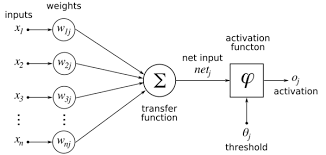
\includegraphics[scale=0.7]{D:/Q2/TFG/data/red_neuronal.png}
\end{center}
\end{figure}


En la parte de la izquierda de la red neuronal se leen los inputs, que, multiplicados por unos pesos se suman. A continuación, mediante una funci\'{o}n de activaci\'{o}n se genera un output, que dependiendo de un número de corte, clasificar\'{a} de una forma u otra los inputs introducidos inicialmente. Pese a tener una estructura definida de una red neuronal, esta era una idea más bien abstracta pues no había ningún método para entrenarla ni generar los pesos del modelo. En otras palabras, no tenía ningún uso pragm\'{a}tico.\\ 


La primera red neuronal entrenable, el \textit{Perceptron}, fue creada en 1957 por el psic\'{o}logo de la universidad de Cornell Frank Rosenblatt. El diseño del \textit{Perceptron} es parecido a una red neuronal actual, aunque solo tiene una capa con pesos y \textit{thresholds} ajustables. El entrenamiento del \textit{Perceptron} se hac\'{i}a de la siguiente forma: 

$$
\begin{aligned}
w_{i} &=w_{i}+\Delta \omega_{i} \\
\Delta w_{i} &=\eta(y-\hat{y}) x_{i} \\
\hat{y} &=\left(\sum_{i} w_{i} x_{i} \geq 0\right)
\end{aligned}
$$


Los pesos se generan de forma aleatoria y se entrenan ajustando el cambio de los pesos ($\Delta w_{i}$) de una iteraci\'{o}n a otra. Mediante el c\'{a}lculo de la variable respuesta (y) menos el valor predicho ($\hat{y}$) por el input ($x_{i}$) y el learning rate ($\eta$) calculamos el cambio en los pesos de la capa. De esta forma iterativamente se va entrenando el \textit{Perceptron} y mediante los pesos de la red este se ajusta a los datos. En este vídeo se explica perfectamente: \href{https://www.youtube.com/watch?v=5g0TPrxKK6o}{perceptron training} \cite{perceptron_train}. \\  


Los \textit{Perceptrones} fueron un \'{a}rea de investigaci\'{o}n hasta que, en 1969 dos investigadores, Marvin Minsky y Seymour Papert, publicaron el art\'{i}culo \textit{Perceptrons} \cite{marvin1969perceptrons} donde se exponía las limitaciones computacionales de la \'{e}poca y la cantidad de tiempo que necesitaban los ordenadores para entrenar estas redes neuronales. 
No fue hasta los años 80 donde la disciplina disfrut\'{o} de un nuevo renacimiento gracias al desarrollo del algoritmo de \textbf{Backpropagation}.\\

Este algoritmo ajusta repetidamente los pesos de las conexiones en la red para minimizar una función (log-loss por ejemplo). El objetivo principal es saber que tan sensible es nuestra funci\'{o}n de coste (la cual queremos optimizar) en relaci\'{o}n con los pesos del modelo. Esto se hace mediante el c\'{a}lculo del descenso de gradiente, un algoritmo con el objetivo de encontrar el m\'{i}nimo local de una funci\'{o}n diferenciable (como podr\'{i}a ser la activaci\'{o}n \textit{logit}: $\mathrm{s}_{(\mathrm{x})}=\frac{1}{1+\mathrm{e}^{-\mathrm{x}}}$).\\

Finalmente, gracias al avance de la industria de los videojuegos, al aumento de la capacidad de procesamiento y al desarrollo de tarjetas gráficas (GPU) se logró una mayor facilidad para entrenar estos algoritmos tan costosos a nivel computacional. \\



El origen del procesamiento del lenguaje natural (NLP) se remonta también a los años 40, despu\'{e}s de la segunda guerra mundial donde cobr\'{o} importancia la capacidad de traducir de un idioma a otro y crear una m\'{a}quina para que lo hiciera era una idea muy alentadora. A lo largo de la segunda mitad del siglo XX se fueron haciendo pequeños pasos, pero ninguno realmente importante. No fue hasta 2013 cuando la disciplina ganó popularidad gracias al desarrollo de \textit{Embeddings}, lo desarrollaremos en la sección \ref{embedding}, y el blog post de Andrej Karparthy \href{http://karpathy.github.io/2015/05/21/rnn-effectiveness/}{\textit{The Unreasonable Effectiveness of Recurrent Neural Networks}} \cite{LSTM_cite} acerca de Redes Recurrentes y las arquitecturas LSTM y GRU. Finalmente, el NLP llegará a su última etapa gracias a las redes \textit{Attention Networks} y modelos como BERT, ERNIE 2.0 y XLNet sustituirán las arquitecturas anteriores. 

\subsubsection{Tipos de NLP en Deep Learning}

En la disciplina del NLP destacan dos grandes ramas con objetivos muy diferentes. La primera gran rama estudia como generar modelos para la clasificación de texto en dos o más categorías, como es nuestro caso. La segunda estudia la generación de texto a partir de texto como podría ser un problema de traducción.\\

Del primero se encarga la disciplina de \textit{NLU} (Natural Language Understanding) que se puede traducir como 
comprensión del lenguaje natural. Algunos modelos de redes neuronales en esta disciplina son: arquitecturas de LSTM, transformer, BERT, RoBerta, Megatron... Tienen como objetivo entender el contexto de una frase para dar una respuesta en forma de categoria. Algunas aplicaciones de estos modelos es el Análisis de Sentimiento en los que podríamos incluir clasificación de opiniones, clasificación de quejas, clasificación de SPAM, etc.\\

En segundo lugar, la rama del NLG (Natural Language Generation) que se puede traducir como generación de lenguaje natural y que incluye modelos como el GPT-II, BART, GPT-III, GShard... Estos modelos tienen como objetivo entender el texto para dar una predicción en forma de secuencia, que en NLP entendemos como texto. Algunas aplicaciones podrían ser chatbots como este llamado \href{https://www.cleverbot.com/}{CleverBot} o traducción de texto como este de \href{https://aws.amazon.com/es/translate/}{amazon}.\\

En este trabajo nos centraremos en la primera disciplina al ser nuestro problema, un problema de clasificación. \\

Para conseguir predecir si una frase es sarc\'{a}stica o no ajustaremos 4 modelos distintos algunos mediante transfer learning y pre entrenados y otros los crearemos enteros y los ajustaremos a la base de datos. Los modelos que entrenaremos ser\'{a}n una red neuronal Convolucional, una red neuronal LSTM (long short-term memory), un modelo BERT con transformadores (el modelo de transformadores para NLU m\'{a}s conocido) y una destilaci\'{o}n del modelo BERT con el objetivo de mejorar los tiempos de entrenamiento. Analizaremos cómo funciona cada modelo y seg\'{u}n la capacidad predictiva que tengan escogeremos uno para resolver el problema. 

\subsection{Arquitecturas y como funcionan}

\subsubsection{Red FCNN (Fully Convolutional Neural Network)}

La primera red neuronal que ajustaremos a la BBDD es una red neuronal Convolucional. Este tipo de redes son de las más usadas en la disciplina del Deep Learning, especialmente para el procesamiento de imágenes y vídeos, aunque también se utilizan para el procesamiento del lenguaje natural.

\paragraph{Capas Convolucionales}

El concepto de una capa Convolucional consiste en procesar un conjunto de datos desplazando o convolucionando (por eso el nombre de estas redes) ventanas o filtros de datos. Estas redes contienen tres parámetros principales. En primer lugar, el número de pasos que avanza en cada iteración. En segundo lugar, el tamaño de la ventana y, por último, el número de ventanas que hay. Cada ventana se multiplica por un conjunto de pesos lo que genera un output. El objetivo de estas redes neuronales subyace en dos ideas principalmente: reducción de parámetros y uso compartido de estos. La reducción de parámetros se logra al generar un output de menores dimensiones que el input. Además de reducir el almacenamiento necesario para la red también se logra mejorar la eficiencia estadística del modelo al regularizarlo. \\

\begin{figure}[h]
\begin{center}
  \caption{Capa Convolucional}
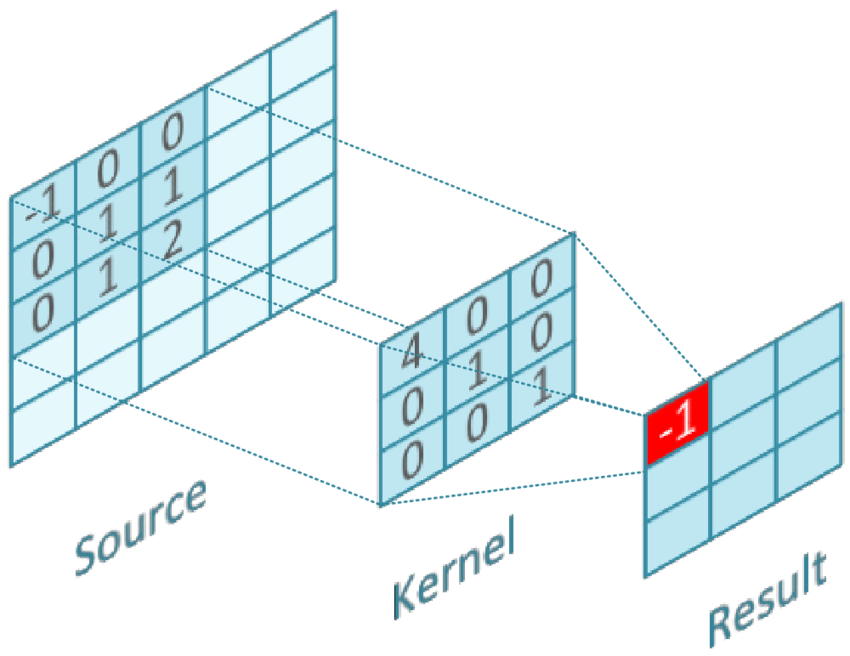
\includegraphics[scale=0.15]{D:/Q2/TFG/data/CNN.png}
\end{center}
\end{figure}





El uso compartido de parámetros se consigue por el kernel mientras que en una red neuronal densa cada input tiene su propio peso. En una red convolucional estos pesos se comparten, lo que reduce a su vez el número de parámetros y produce que zonas cercanas tengan parámetros compartidos.  Lo podemos visualizar mejor en la siguiente imagen:\\ 


\begin{figure}[h]
\begin{center}
  \caption{Kernel CNN}
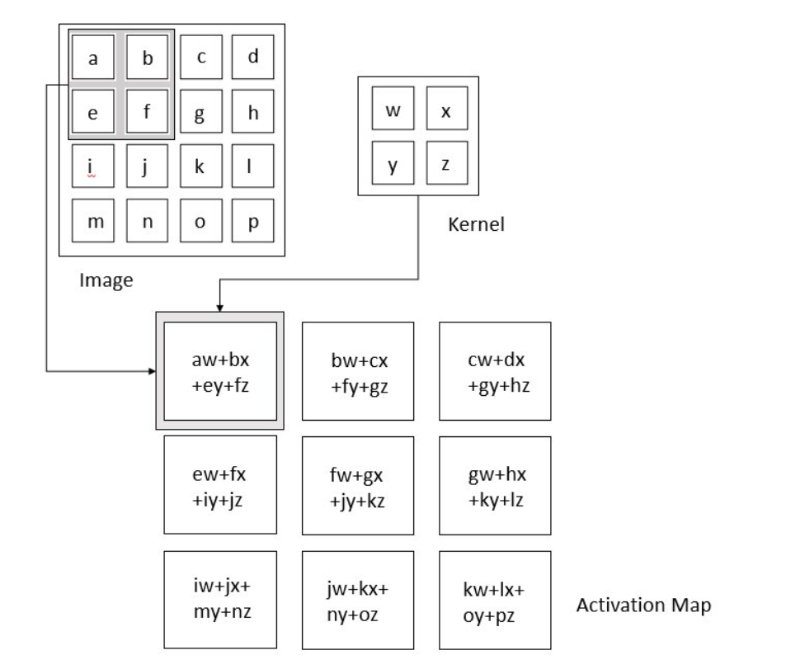
\includegraphics[scale=0.4]{D:/Q2/TFG/data/kernel_CNN.png}
\end{center}
\end{figure}


Una red convolucional funciona de forma parecida al córtex cerebral. Mediante la activación de muchas neuronas con ciertos patrones en los datos, conseguimos crear abstracciones más complejas.\\

Además de las capas convolucionales también existen otros componentes en la red neuronal que permiten optimizar el resultado de estas redes. 

\paragraph{Embeddings\\}



Uno de estos componentes son los embeddings. Un embedding es una \label{embedding} representación vectorial de baja dimensionalidad de variables discretas. Este crea un vector de números reales para reducir la dimensionalidad de una variable categórica y darle un significado en el espacio transformado. \\

De esta forma conseguimos que palabras con significados parecidos tengan una representación vectorial, en X dimensiones, similar. Así se evita el \textit{one-hot encoding}, utilizado para modelar variables categóricas y que en un problema de NLP crearía millones de dimensiones. El funcionamiento de un embedding se puede entender con el siguiente ejemplo: la palabra \textit{Reina} tendrá un vector muy parecido a la suma de los vectores \textit{Rey - hombre + mujer}.  De esta forma, los embeddings traducen de cierta manera el significado que le damos los humanos a las palabras al lenguaje de un ordenador.\\

La utilización de embeddings se puede hacer:
\begin{itemize}

\item{Entrenando el embedding con la red neuronal añadiendo una capa con X dimensiones, para que aprenda utilizando el algoritmo de Backpropagation.}

\item{Mediante transfer Learning, es decir, importar un embedding ya entrenado (como en nuestro caso \label{GloVe}\textit{GloVe}).\footnote{GloVe es una representación vector de palabras desarrollado por Jeffrey Pennington con técnicas de factorización de matrcies y Análisis semántico latente (LSA) Mas información en el \href{https://nlp.stanford.edu/pubs/glove.pdf}{paper}.\cite{LSA}}}


\end{itemize}

A parte del uso que le hemos dado en este trabajo los embeddings también se pueden utilizar para la visualizar relaciones entre variables y la creación de clústers.\clearpage


\begin{figure}[h]
\caption{Creación de clústers mediante embeddings}
\begin{center}
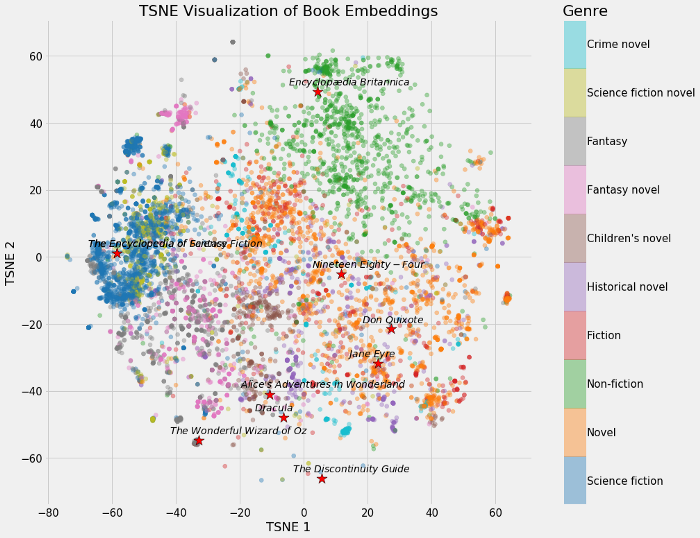
\includegraphics[scale=0.2]{D:/Q2/TFG/data/embeddings_visualization.png}
\end{center}
\end{figure}

No entraremos en más detalle porque esta fuera del objetivo de este trabajo, pero en este \href{https://towardsdatascience.com/visualizing-feature-vectors-embeddings-using-pca-and-t-sne-ef157cea3a42}{artículo} \cite{visualization_word_embedd} se puede entrar más en profundidad.

 
\paragraph{Dropout}

\label{drop}
Las redes neuronales son algoritmos de Machine Learning muy potentes, sin embargo, el sobre ajuste a los datos de entrenamiento, especialmente en una base de datos pequeña, es un problema. Para evitarlo utilizamos la capa \textbf{Dropout}, esta capa elimina con probabilidad \textit{p} cada neurona y todos sus nodos. De esta forma, conseguimos regularizar el modelo y por tanto la inferencia de este es mejor.


\begin{figure}[h]
\begin{center}
  \caption{Capa Dropout}
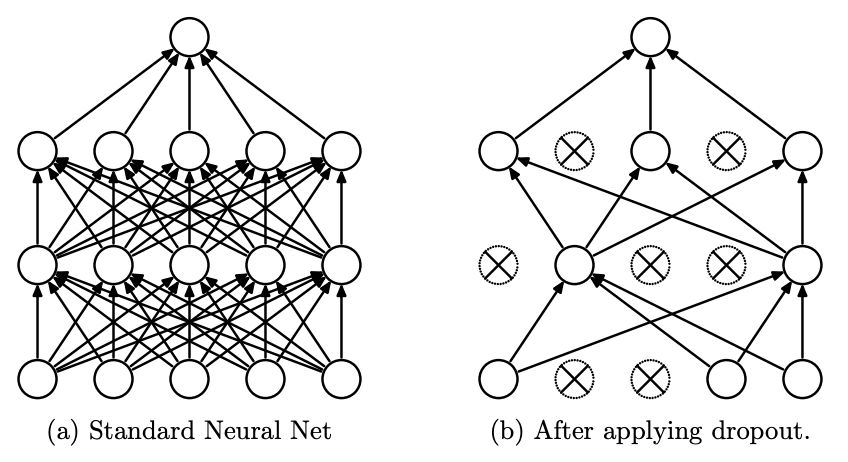
\includegraphics[scale=0.4]{D:/Q2/TFG/data/dropout.png}
\end{center}
\end{figure}

Se puede encontrar más información en el siguiente articulo: \href{https://leimao.github.io/blog/Dropout-Explained/}{Dropout Explained} \cite{dropout}


\paragraph{Batch Normalization}

\label{batch}

La capa de \textbf{Batch normalization} tiene la función de estandarizar los inputs de una capa. De esta forma, la distribución de los inputs no cambia, lo que deriva en menores tiempo de entrenamiento y regularización de la red neuronal lográndose una mejor generalización del modelo. 
 
\paragraph{Global Max Pooling}

\label{MaxPool}

La capa Global Max Pooling reduce el número de dimensiones de la capa de entrada. Lo que hace esta capa es coger el máximo de entre un conjunto de vectores. De esta forma, reducimos el número de parámetros además de regularizar la red neuronal. Se puede entender mejor mediante esta imagen : 


\begin{figure}[h]
\begin{center}
  \caption{Global Max Pooling}
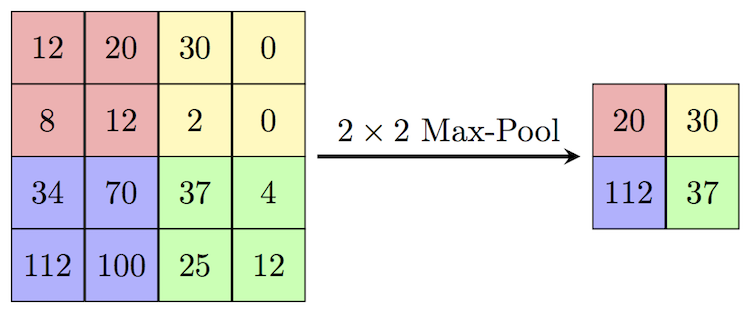
\includegraphics[scale=0.8]{D:/Q2/TFG/data/global_max.png}
\end{center}
\end{figure}

Se puede encontrar más información el siguiente \href{https://arxiv.org/pdf/1908.05040.pdf}{paper} \cite{MaxPool}

\paragraph{Estructura de la red neuronal}

Los componentes previamente comentados se ordenan de la siguiente forma para conseguir la máxima capacidad predictiva posible, obteniendo el modelo siguiente:

\label{red_FCNN}


\begin{figure}[h]
\begin{center}
  \caption{Modeo Fully Convolutional Network}
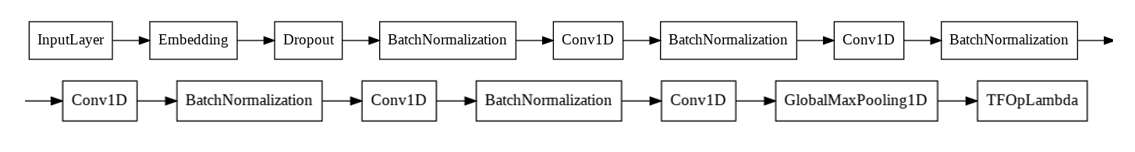
\includegraphics[scale=0.5]{D:/Q2/TFG/data/modelo_FCNN.png}
\end{center}
\end{figure}



Ahora falta ajustar los datos a la estructura de \textit{Tensorflow} para que la red los pueda entender, entrenar el modelo y testear que funcione correctamente. 


\subsubsection{Red LSTM (Long Short-Term Memory)}

\paragraph{Capa LSTM}

Esta arquitectura comparte todos los componentes de la arquitectura anterior, es decir, los embeddings descritos en la sección \ref{embedding}, Dropout en la sección \ref{drop}, Batch Normalizatión en \ref{batch} y Global Max Pooling en la sección \ref{MaxPool}. Sin embargo, las capas convolucionales son sustituidas por capas LSTM. Estas son un tipo especial de red recurrente\footnote{Las redes recurrentes se diferencian del resto en que incorporan retroalimentación lo que permite crear temporalidad.} (RNN), inventadas en 1997 por Sepp Hochreiter y Jürgen Schmidhuber. Tienen como objetivo principal solucionar el problema de este tipo de redes: memoria corta.\\

Para hacerlo, se usa una estructura de puertas que retiene o elimina diferentes segmentos de una frase según la importancia que tiene. Por ejemplo, imaginemos que queremos predecir si una opinión es buena o mala y tenemos la frase siguiente:

\begin{itemize}
\item{Este libro acerca de Machine Learning no me ha servido para nada}
\end{itemize} 

La red neuronal aprenderá qué palabras de la frase son importantes para la predicción y cuales no. En este caso se quedaría con la parte en negrita:

\begin{itemize}
\item{\textit{Este libro acerca de Machine Learning} \textbf{no me ha servido para nada}}
\end{itemize} 

Para conseguirlo usamos la siguiente estructura:\\


\begin{figure}[h]
\begin{center}
  \caption{Estructura de una célula LSTM}
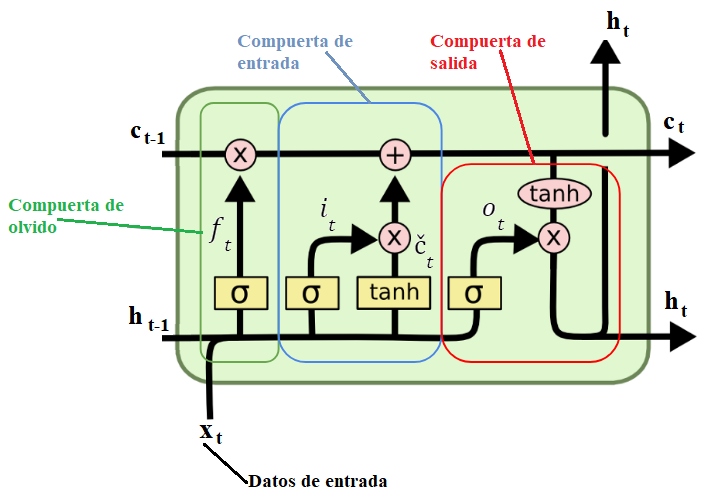
\includegraphics[scale=0.3]{D:/Q2/TFG/data/LSTM.png}
\end{center}
\end{figure}


En la primera parte juntaremos el \textit{hidden state}\footnote{El hidden state se puede entender como una caracterización de la palabra t-1} ($h_{t-1}$) y la nueva palabra $X_{t}$. Que pasará por la \textit{forget gate} que mediante una función de activación \textit{sigmoid}\footnote{La función de activación \textbf{sigmoid}, da números entre 0 y 1 y tiene la forma: $$ h_{x} =  \frac{\mathrm{1} }{\mathrm{1} + e^{-x} }  $$} nos dará un output que llamaremos $F_{t}$. A continuación, la combinación ($\textit{hidden state} + X_{t}$) pasará por la función Input gate. Pasará por la función sigmoid que dará un output el cual podemos llamar $I_{t}$ y paralelamente por la función \textit{tanh}\footnote{La función tanh da valores entre 1 y -1 y tiene la forma: $$\sigma(z)=\frac{e^{z}-e^{-z}}{e^{z}+e^{-z}}$$} que dará un output que llamaremos $\hat{c}$ (candidate). Estos dos outputs los multiplicaremos y lo sumaremos a la multiplicación de la Cell State\footnote{El Cell state se puede entender como una agregación de lo que hemos aprendido en la secuencia} ($C_{t-1}$) por $F_{t}$ que hemos obtenido de la \textit{forget gate}. Es decir: $ C_{t} = C_{t-1} * F_{t} + I_{t} * \hat{c} $. Por último, pasamos la primera combinación ($h_{t-1} + X_{t}$) por la función \textit{sigmoid} de la zona 3 y paralelamente la Cell State ($C_{t}$ por la función \textit{tanh} multiplicamos los resultados que nos dará la nueva \textit{hidden state}($h_{t}$). Pasaremos la \textit{Cell State} y el \textit{hidden state} a la siguiente parte de la secuencia. También se puede entender en forma de código:\\


\begin{figure}[h]
  \caption{Estructura de una célula LSTM en código}
\begin{center}
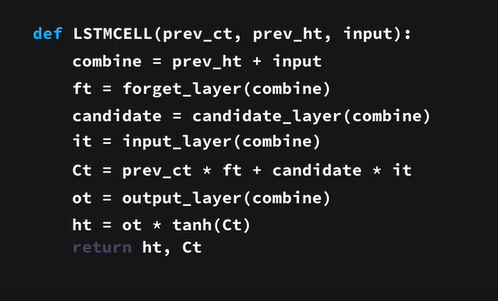
\includegraphics[scale=0.5]{D:/Q2/TFG/data/LSTM_codigo.png}
\end{center}
\end{figure}


Este vídeo \href{https://www.youtube.com/watch?v=8HyCNIVRbSU}{vídeo} \cite{LSTM_explanation} lo ilustra perfectamente. 


\paragraph{Estructura de la red neuronal}
Finalmente, y con una estructura parecida a la arquitectura de la red FCNN en la sección \ref{red_FCNN}, sustituyendo por capas Densas creamos el siguiente modelo:

\label{LSTM_model}
\begin{figure}[h]
  \caption{Estructura del modelo LSTM}
  \begin{center}
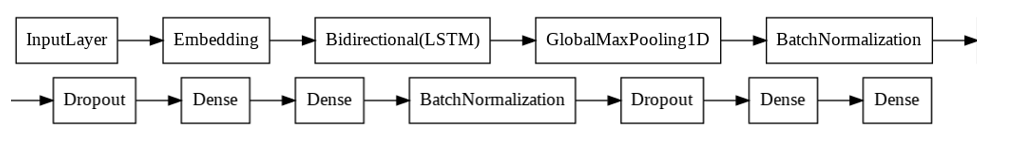
\includegraphics[scale=0.5]{D:/Q2/TFG/data/LSTM_architecture.png}
\end{center}
\end{figure}


\subsubsection{Modelo BERT y transformadores}

\paragraph{Breve introducción a los tranformadores}

El modelo BERT nace de una subclase de redes neuronales llamados \textit{transformers} o modelos de atención. Estos nacieron para solventar los problemas que generan modelos de redes convolucionales y especialmente las redes recurrentes (RNN), sobre todo las arquitecturas LSTM y GRU\footnote{La arquitectura GRU es muy parecida a la arquitectura LSTM y su objetivo principal es simplificar los modelos LSTM para conseguir entrenamientos más rápidos, estas dos arquitecturas consiguen resultados comparables}.\\

 El principal beneficio del modelo BERT con respecto otras arquitecturas de redes recurrentes es que ignora el orden de las palabras. Esto permite paralelizar el proceso de entrenamiento de la red neuronal en varios clústers y, en consecuencia, acelerar el proceso de entrenamiento evitando cuellos de botella. Además, consigue captar la relación entre dos partes distantes entre sí, que con modelos LSTM tienden a subestimarse.\\
 
Las principales desventajas de estas arquitecturas es que son muy intensivas computacionalmente además de necesitar bases de datos muy grandes y, por tanto, un presupuesto elevado para entrenarlas. \\

En su origen, se desarrollaron para tareas \textit{sequence to sequence}, lo que en el campo del NLP se entendería como generar texto a partir de otro texto (NLG). Por esto, este tipo de redes neuronales son muy útiles para tareas de traducción de texto, resumen de texto o chatbots entre otros. Sin embargo, estos también se pueden utilizar como embeddings, tema que comentamos en la sección \ref{embedding}, y que son perfectos para problemas de clasificación como el nuestro. \\

Y es que el origen de la estructura de un modelo trasformer es el siguiente: 


\begin{figure}[h]
\begin{center}
  \caption{Estructura de un modelo transformer}
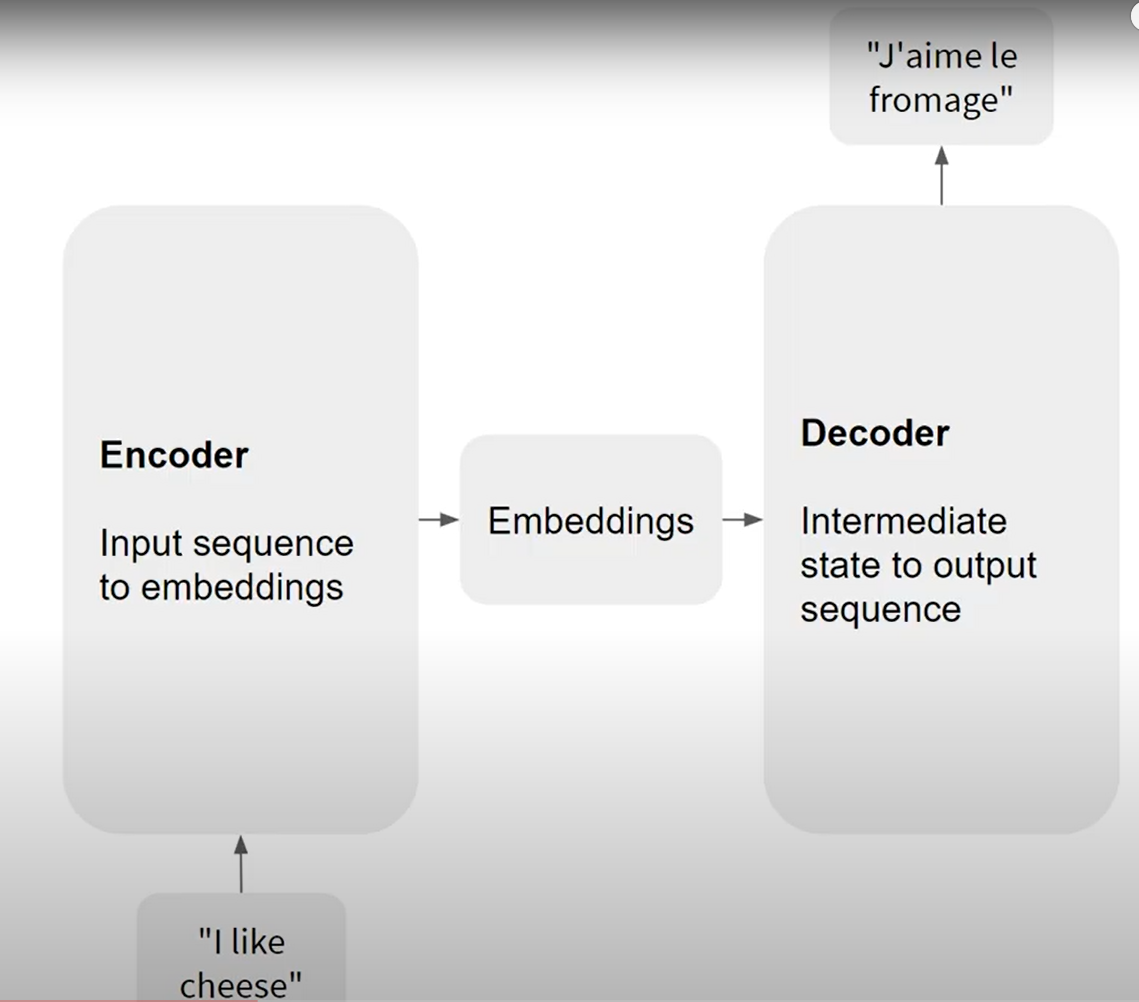
\includegraphics[scale=0.15]{D:/Q2/TFG/data/trasnformers.png}
\end{center}
\end{figure}


En primer lugar, un codificador genera un embedding (es decir una representación numérica), a partir de una secuencia, en nuestro caso una frase,  y después un descodificador crea el output a partir del embedding creado por la primera parte de la arquitectura. Este codificador se genera mediante el apilamiento de \textit{Multiheaded self attention modules}. Estos módulos tienen la estructura siguiente: 

\begin{figure}[h]
  \caption{Arquitectura de Módulos de autoatención de múltiples kernels}
  \begin{center}
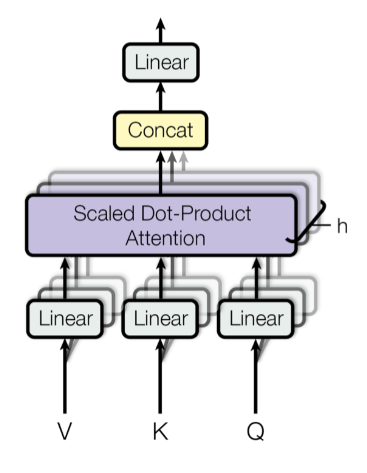
\includegraphics[scale=0.35]{D:/Q2/TFG/data/attention_mechanism.png}
\end{center}
\end{figure}


En primer lugar, como input tendremos las matrices V (value), K (key) y Q (query). Estas tres matrices se pueden entender como un sistema de búsqueda. La matriz Q sería la palabra que buscamos, la matriz K es el conjunto de candidatos de esa búsqueda y finalmente V son los resultados que mejor se ajustan a la búsqueda. Cada una de estas matrices es el resultado de un conjunto de pesos por la matriz input, es decir: 

$$
\begin{gathered}
\text { query }=\boldsymbol{W}^{q} \boldsymbol{x}_{i} \\
\text { key }=\boldsymbol{W}^{k} \boldsymbol{x}_{i} \\
\text { value }=\boldsymbol{W}^{v} \boldsymbol{x}_{i}
\end{gathered}
$$


A continuación, estas matrices se procesarán mediante \textit{Scaled Dot-Product Attention}. Este mecanismo de atención tiene la estructura siguiente: 

\begin{figure}[h]
  \caption{Estructura de un módulo de atención}
  \begin{center}
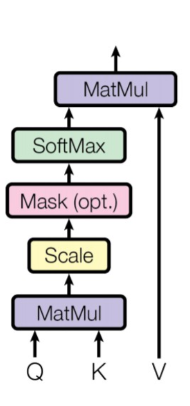
\includegraphics[scale=0.3]{D:/Q2/TFG/data/dotted_attention.png}
\end{center}
\end{figure}




Del que se obtiene el resultado de la siguiente función: $$
A(Q, K, V)=\operatorname{softmax}\footnote{La función softmax es una función que convierte un vector de K valores reales en un vector de K valores reales que suman 1. Los valores de entrada pueden ser positivos, negativos, cero o mayores que uno, pero softmax los transforma en valores entre 0 y 1, para que puedan interpretarse como probabilidades. Tiene la forma $\sigma(\vec{z})_{i}=\frac{e^{z_{i}}}{\sum_{j=1}^{K} e^{z_{j}}}$
}\left(\frac{Q K^{\top}}{\sqrt{d_{k}}}\right) V
$$ 

Donde $\sqrt{d_{k}}$ es el tamaño del embedding. Tanto las matrices V,K,Q como el \textit{Scaled Dot-Product Attention} se ejecuta de forma paralelizada, lo que genera h vectores que se concatenan. \\

Finalmente, el encoder-decoder tendrá una estructura como esta: 


\begin{figure}[h]
  \caption{Estructura global modelo transformer}
  \begin{center}
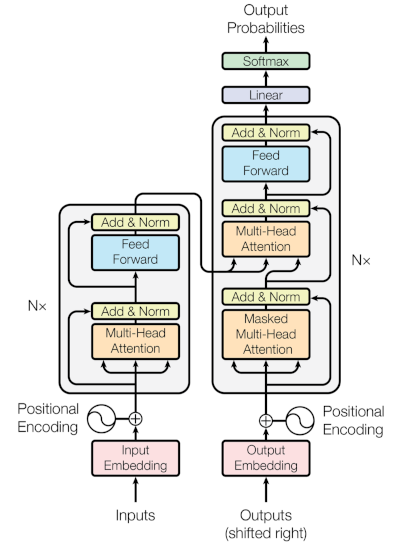
\includegraphics[scale=0.3]{D:/Q2/TFG/data/estructura_transformers.png}
\end{center}
\end{figure}



Se puede encontrar más información en el paper original \href{https://arxiv.org/abs/1706.03762?context=cs}{\textit{attention is all you need.}} \cite{Attention}. También, el siguiente vídeo lo explica muy bien: \href{https://www.youtube.com/watch?v=KN3ZL65Dze0}{NLP for Developers: Transformers | Rasa} \cite{transformers}.

\paragraph{BERT}



El modelo BERT (Bidirectional Encoder Representation from
\label{BERT} Transformers) fue publicado por investigadores de Google en el año 2019 para modelar el lenguaje natural (NLP). Las tareas en las cuales destaca son: análisis de sentimiento, análisis de rol semántico, clasificación de textos,... Y, por tanto, es perfecto para nuestro problema (Sentiment Analysis). El modelo BERT es entrenado de dos formas con objetivos distintos. En primer lugar, BERT debe predecir palabras escondidas aleatoriamente en la misma frase. En segundo luagr, BERT debe predecir si el siguiente trozo de texto formaba parte de la oración original o ha sido cambiada por un trozo aleatorio.\\

El objetivo de predecir palabras faltantes o escondidas (MLM, Masked Language Model) mediante el resto de las palabras permite al modelo generar un contexto. Esto consigue que una palabra no se entienda con ella sola, es decir que el significado de la palabra este condicionada por el contexto de la frase. Por otro lado, el objetivo de predecir el siguiente trozo de texto es enseñar al modelo a definir si dos trozos de texto tienen relación entre sí o no. Una de las ventajas de este método de entrenamiento reside en la tipo de base de datos necesaria para entrenarla, que, al no estar etiquetada se puede entrenar de forma auto supervisada.\\ 

BERT fue preentrenado usando únicamente texto, concretamente fue entrenado con el conjunto de texto de Wikipedia. Esta capacidad de entrenamiento con millones de datos contrasta con embeddings como \textit{GloVe}, del cual hablamos en la sección \ref{GloVe}. Se puede encontrar más información en el \href{https://arxiv.org/abs/1810.04805}{paper} \cite{BERT} original: \\

En nuestro problema clasificación de texto, BERT se utiliza como un Embedding y, mediante transfer learning, cargamos los pesos del modelo, los cuales no se entrenarán y se congelarán. Finalmente quedará el siguiente modelo: 


\begin{figure}[h]
  \caption{Estructura de nuestro modelo con BERT}
  \label{BERT_model}
  \begin{center}
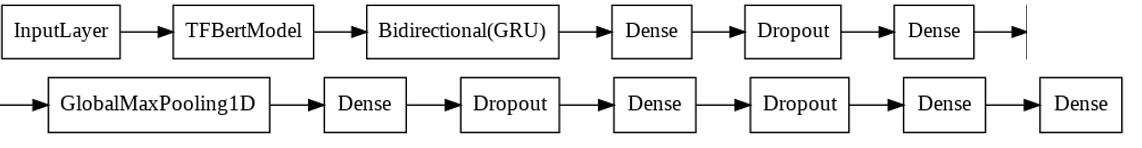
\includegraphics[scale=0.5]{D:/Q2/TFG/data/BERT_model.png}
\end{center}
\end{figure}


Como vemos el módulo BERT ha sido acompañado con una capa GRU que, como comentamos anteriormente de forma breve, es una capa Recurrente muy parecida a la capa LSTM y algo más simple. A esto, se le añade un conjunto de capas \textit{Densas, Dropout y Max Pooling} organizados alternativamente que finalmente acaba en una activación \textit{sigmoid}. \\
 

La estructura del módulo BERT \cite{evolved_transformer}, BERT \textbf{base} en nuestro caso, es la siguiente: 


\begin{figure}[h]
\caption{Estructura de BERT}
\begin{center}
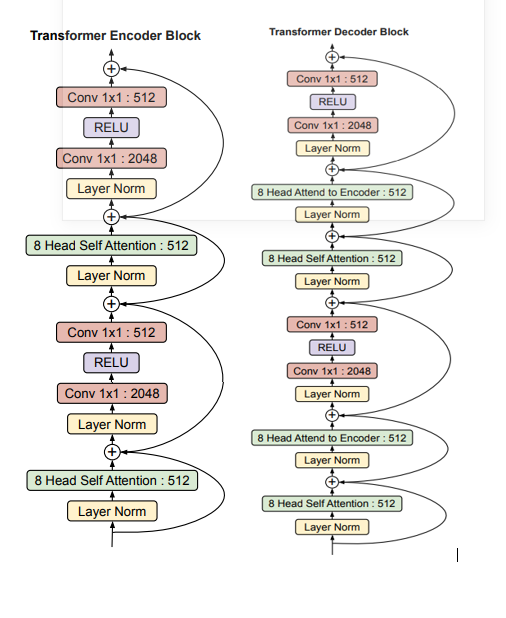
\includegraphics[scale=0.3]{D:/Q2/TFG/data/BERT_structure.png}
\end{center}
\end{figure}

Esta tiene una gran cantidad de parámetros, lo que resulta muy costoso de entrenar y el tiempo de inferencia es muy elevado... Es por eso por lo que han surgido técnicas para reducir el número de parámetros sin reducir, en la medida de lo posible, el rendimiento de la arquitectura. Y de esta forma, se consigue adaptar estos modelos a dispositivos más pequeños como móviles, cámaras o dispositivos IoT. 

\paragraph{Reducción de parámetros y peso de un modelo BERT}

\subparagraph{Pruning\\}

El \textit{Pruning} es uno de los métodos para reducir el número de parámetros y agilizar el tiempo de inferencia de estos modelos. Este se basa en la idea de que muchos modelos están sobre parametrizados y, por lo tanto, se pueden eliminar conexiones y sus pesos correspondientes sin que haya un descenso en el rendimiento del modelo e incluso, puede ayudar a regularizar el modelo y que generalice mejor.

\subparagraph{Quantization\\}

\textit{Quantization} es un método para reducir el peso de los parámetros. Consiste en aproximar los pesos a un menor de número de decimales y, de esta forma, se acelera el proceso de inferencia y consiguiéndose reducir el coste en memoria del modelo. Si comparamos los tipos Float32 vs INT8, reducimos el almacenamiento de los datos y del modelo cuatro veces. 

\subparagraph{Distillation\\}

La destilación de una arquitectura es la simplificación de un modelo más grande eliminando partes de la estructura. De esta forma, se acerca lo máximo posible al modelo inicial o profesor, intentando evitar una pérdida grande en el rendimiento del modelo.\\

Algunos modelos de Prunning, Quantization, Distillation basados en BERT son los siguientes: \cite{arquitecturas}

\begin{figure}[h]
\caption{Diferentes modelos de reducción de tamaño}
\begin{center}
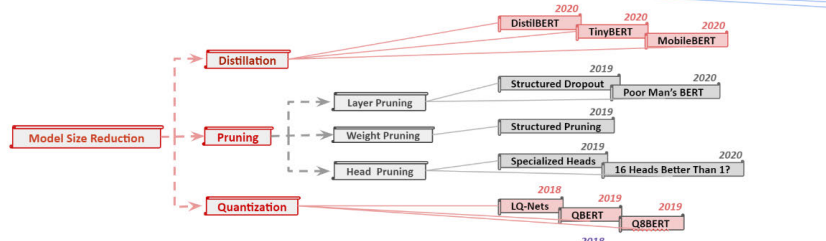
\includegraphics[scale=0.7]{D:/Q2/TFG/data/model_size_reduction.png}
\end{center}
\end{figure}

Continuaremos por esta línea, aplicando un modelo DistilBERT a nuestro conjunto de datos para agilizar el proceso de entrenamiento y terminando con los 4 modelos que ajustaremos a nuestra base de datos. 


\subsubsection{El modelo DistilBERT} 

El modelo DistilBERT es un modelo cuyo tamaño se reduce hasta un 40\% (con respecto BERT) y un 60\% más rápido. Este fue creado con dos metas principales, en primer lugar, reducir el impacto medioambiental como consecuencia del escalado continuo en el número de parámetros y, por tanto, de la energía para entrenarlos. Y, en segundo lugar, habilitar a dispositivos con menos potencia computacional, principalmente móviles, a usar estos modelos para inferencia. \\

Según los autores \textbf{Distilbert} \cite{distilBERT} es capaz de retener un 97\% de la precisión en tareas de clasificación del modelo original \textbf{BERT} que explicamos en la sección \ref{BERT}.\\

Estos resultados están basados en GLUE (General Language Understanding Evaluation), que contiene 9 bases de datos para evaluar sistemas de comprensión del lenguaje natural. Más información en enlace siguiente \href{https://gluebenchmark.com}{GLUE}. \\

Finalmente, generamos un modelo muy parecido al BERT, aunque algo menos regularizado:

\begin{figure}[h]
\caption{Modelo Distilbert}
\begin{center}
  \label{distilBERT_model}
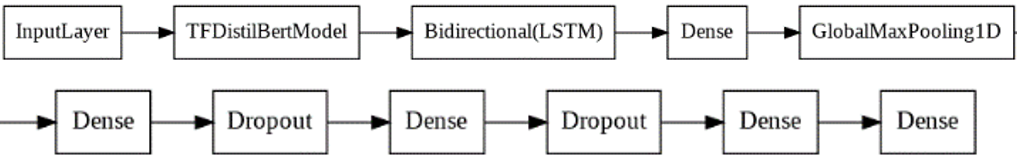
\includegraphics[scale=0.5]{D:/Q2/TFG/data/distilbert_structure.png}
\end{center}
\end{figure}







% \begin{figure}
 %\caption{Tipos de modelos NLP}
%\includegraphics[scale=0.2]{D:/Q2/TFG/data/%clasificacion_modelos_NLP.PNG}
%\end{figure}


\section{Marco pr\'{a}ctico}

\subsection{Análisis Exploratorio de la base}

Antes de ajustar ningún modelo o crear un preprocesamiento de los datos primero analizaremos las características de la base para poder solucionar problemas inherentes en la base. \\

La base tiene un tamaño de 20.033 filas y dos columnas, el texto y la respuesta. No tiene nulos en ninguna de las columnas y por tanto no habrá que desestimar ninguna fila. Hay un 47\% de frases \textbf{no} sarcásticas y por tanto 53\% de frases que, si lo son, en otras palabras, la variable respuesta esta balanceada así que no habrá que hacer \textit{Data Augmentation}\footnote{Las técnicas de aumento de datos se utilizan para generar datos sintéticos adicionales utilizando los datos que tiene} o \textit{Downsampling}\footnote{La reducción de muestreo es un mecanismo que reduce el recuento de muestras de entrenamiento que caen dentro de la clase mayoritaria.}. \\

La longitud de las frases mediano en caracteres es 60 además observamos un outlier muy claro que tiene más de 800. En la figura~\ref{fig:Distribucion_ch} podemos ver tanto la distribución con el outlier como sin él. Parece que exceptuando el outlier la distribución es relativamente simétrica. 


\begin{figure}[h]
\caption{Distribución de caracteres}
\begin{center}
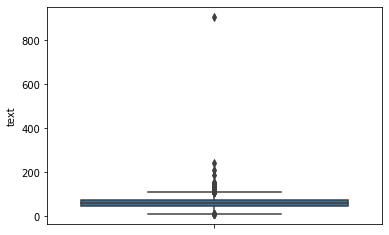
\includegraphics[scale=0.5]{D:/Q2/TFG/data/distrib_caracteres.png}
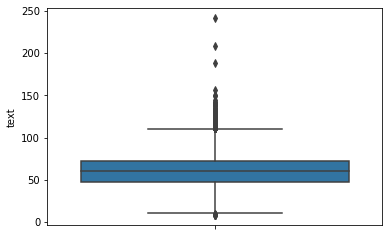
\includegraphics[scale=0.5]{D:/Q2/TFG/data/distrib_caracteres_no_out.png}
\label{fig:Distribucion_ch}
\end{center}
\end{figure}


La longitud de las frases mediano en palabras es 10 aunque, y otra vez, hay 1 outlier muy claro que tiene más de 140 palabras, es la misma frase. En la figura~\ref{fig:Distribucion_w} podemos ver tanto la distribución con el outlier como sin él. Parece que exceptuando el outlier la distribución es, otra vez, relativamente simétrica. 


\begin{figure}[h]
\caption{Distribución de palabras}
\begin{center}
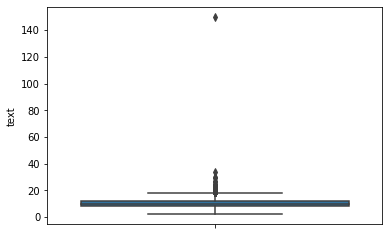
\includegraphics[scale=0.5]{D:/Q2/TFG/data/distrib_words.png}
\label{fig:Distribucion_w}
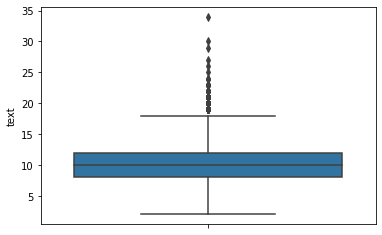
\includegraphics[scale=0.5]{D:/Q2/TFG/data/distrib_words_no_out.png}
\end{center}
\end{figure}

Con esta información ajustaremos el número de palabras que cogeremos por frase a 20, haciendo un \textit{padding}\footnote{Las redes neuronales necesitan que todas las filas contengan el mismo número de palabras, para ello añadimos valores no relevantes para la red neuronal para tener el mismo número de palabras por fila.} de 0 si la frase fuera más corta. \\

Además, para entender un poco más nuestra base de datos visualizaremos cuales son las palabras más repetidas por categoría. 

\begin{figure}[h]
\caption{Palabras más repetidas}
\begin{center}
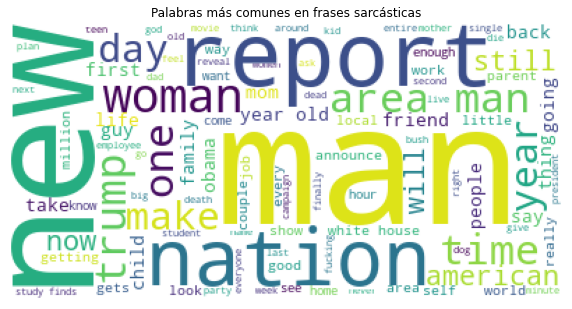
\includegraphics[scale=0.36]{D:/Q2/TFG/data/frases_sarcasticas.png}
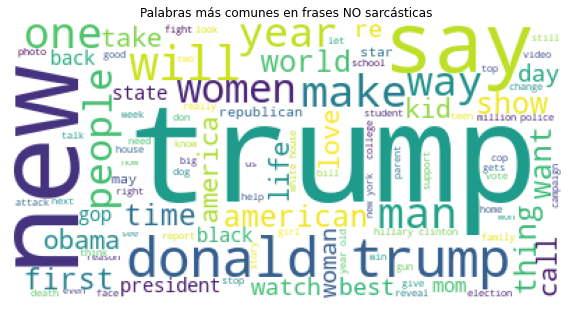
\includegraphics[scale=0.36]{D:/Q2/TFG/data/frases_no_sarcasticas.png}
\end{center}
\end{figure}

De estos gráficos se puede extrapolar que el tema predominante es la política americana. En cuanto a diferencias entre las dos categorías observamos que la palabra \textbf{Donald Trump} es mencionado muchas veces en la categoría: no sarcástica. A parte de esto no podemos ver grandes diferencias entre ambos gráficos, lo que reafirma la necesidad de un algoritmo de \textit{machine learning} debido a la complejidad del problema.

\subsection{Prepocesamineto de la base de datos}

Para que los modelos ajusten con corrección debemos aplicar anteriormente una fase de preprocesamiento y de esta forma, optimizar el proceso de entrenamiento del modelo. En los casos de las redes neuronales \hyperref[red_FCNN]{FCNN} y \hyperref[LSTM_model]{LSTM} el preprocesamiento será compartido. Por otro lado, en el caso de los modelos conseguidos mediante \textit{transfer learning} el preprocesamiento se hará con un \textit{tokenizer}\footnote{Un tokenizador divide los datos no estructurados y el texto en lenguaje natural en fragmentos de información que pueden considerarse elementos discretos.} importado de la libreria \code{transformers}.

\subsubsection{Preprocesamiento para los modelos LSTM y FCNN}

\label{preproc_LSTM_FCNN}

Antes de nada, dividiremos la base en tres: entrenamiento, la validación y test. La primera se utiliza para entrenar el modelo, la segunda para optimizar los hiperparámetros del modelo y la última para comprobar que el modelo funciona correctamente.\\ 

Para empezar con la limpieza de la base haremos uso de las \textit{stopwords}. Es decir, eliminaremos palabras que no aporten gran valor a una oración, como artículos o verbos auxiliares. A continuación, eliminamos la puntuación, caracteres especiales y saltos de línea. \\

Continuamos, tokenizando las palabras, asignando a cada palabra distinta un número entero. En nuestro caso cogeremos un total de 10.000 palabras distintas, el resto por lo tanto no tendrán un número entero \textbf{único} asignado. \\

Por último, y como hemos dicho en la sección anterior, cogemos 20 palabras. Si la frase fuera más larga la cortaríamos y si fuera más corta añadiríamos ceros hasta llegar 20 números por fila. 

\subsubsection{Preprocesamiento para los modelos BERT y distilBERT}

Para los modelos BERT y distilBERT nos bajaremos el tokenizador de   la librería \code{transformers}. A continuación, usamos la función \code{encode\_plus} de la misma librería. Esta función nos hace el padding del dataset además nos asigna un número a cada palabra y un vector de \textit{masks}. Estos \textit{masks} de atención son necesarios para decirle al modelo (BERT) a qué id de entrada deben prestarse atención y cuáles no.\\

Por último, cargamos la base a un dataset de tensores de Tensorflow para optimizar la carga de los datos y dividimos la base en entrenamiento, validación y testing. 


\subsection{Componentes en el entrenamiento de una red neuronal}


Para entrenar los modelos de forma óptima ajustamos los hiperparámetros del modelo para acelerar el entrenamiento y regularizar la red neuronal. De esta forma, reducimos el tiempo de entrenamiento y el número de épocas\footnote{El número de épocas es un hiperparámetro de descenso de gradiente que controla el número de pases completos a través del conjunto de datos de entrenamiento.} que necesitamos para entrenarlo. Además, evitaremos que sobreajuste. \\

Para ello, y como hemos explicado brevemente, utilizaremos la base de datos de validación. De esta forma para cada época iremos ajustando hiperparámetros del modelo. Para entrenar la base de datos usamos el optimizador\footnote{Los optimizadores son algoritmos o métodos que se utilizan para cambiar los atributos de la red neuronal, como los pesos y el Learning Rate, para minimizar una función en nuestro caso el log-loss} \textbf{Adam} y la función que minimizamos es la log-loss \footnote{Log-loss es indicativo de qué tan cerca está la probabilidad de predicción del valor real/verdadero correspondiente (0 o 1 en caso de clasificación binaria). Cuanto más diverja la probabilidad predicha del valor real, mayor será el valor de pérdida logarítmica.}.\\

También añadiremos el componente de \textbf{Early Stopping}. Este, parará el proceso de entrenamiento si en un número predefinido de épocas el log-loss no mejora en la validación. Al acabar, el componente reajustará los pesos que mejor han funcionado en la base de validación. \\

Por último, añadiremos el componente de \textbf{Warmup}. El \textbf{Warmup} reducirá el Learning Rate en la primera o las primeras épocas. Después de las primeras épocas, utiliza el Learning Rate ''regular''. Se ha comprobado que comenzar lentamente calibra módulos como los mecanismos de atención en la red. Es por ello por lo que esta técnica se utiliza sobre todo en arquitecturas de transformadores. 


\subsubsection{Métricas}

Como métricas para saber cómo está funcionando nuestro modelo utilizaremos cinco: El log-loss, la precisión, el F1, la especificidad y la sensibilidad. El log-loss nos dice como ajusta el modelo a la base (tanto si acierta como si no), la precisión es el porcentaje de aciertos que tenemos. La especificidad es el \% de aciertos en la categoría negativa y se calcula mediante $ especificidad = \frac{VN}{VN + FP} $ donde VN = verdadera negativo y FP = falso positivo.  La sensibilidad es el \% de aciertos en la categoría positiva y se calcula mediante $ Sensibilidad = \frac{VP}{VP + FN} $ donde VP = verdadera positivo y FN = falso negativo.  El F1 es una medida que penaliza si la especificidad y la sensibilidad están muy descompensadas lo que indicaría que estamos prediciendo muy bien una categoría a costa de la otra. La fórmula es la siguiente: $$
F 1=\frac{2 \times \text { especificidad } \times \text { Sensibilidad }}{\text { especificidad }+\text { Sensibilidad }}
$$


\subsection{Resultados}

\subsubsection{Modelo FCNN}

El modelo \hyperref[red_FCNN]{FCNN} ha funcionado bastante bien. Ha obtenido,en el testing dataset, un log-loss de \textbf{0.363}, un acierto del \textbf{85,26 \%}, una sensibilidad del \textbf{83,6 \%}, una especificidad del \textbf{85,1 \%} y por tanto un F1 de \textbf{84,4 \%}. \\

El proceso de entrenamiento ha sido muy rápido (8-9 segundos por época) y las métricas han convergido de la siguiente forma: 

\begin{figure}[h]
\caption{Resultados modelo FCNN}
\begin{center}
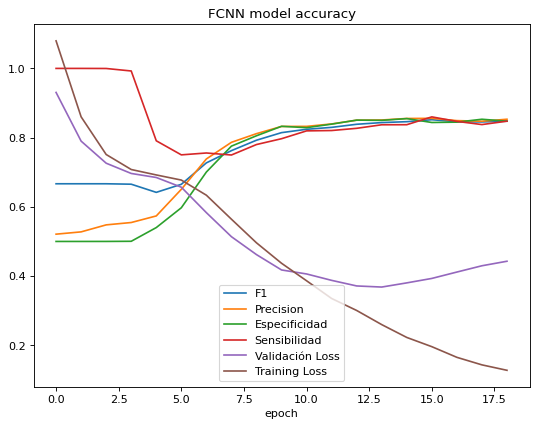
\includegraphics[scale=0.3]{D:/Q2/TFG/data/FCNN_results.png}
\end{center}

\end{figure}

Observamos como la sensibilidad, la especificidad, el F1 y la precisión van convergiendo hacia el 84\% aproximadamente. Además, vemos como se ha generado un codo entre el validation loss y el training loss hacia la época 13 donde el validation loss ya no mejora. Es decir, el modelo empieza a sobre ajustar .

\subsubsection{Modelo LSTM}

El modelo \hyperref[LSTM_model]{LSTM} ha funcionado ha funcionado algo peor que el modelo FCNN. Ha obtenido, en el testing dataset, un log-loss de \textbf{0.369}, un acierto del \textbf{84,03 \%}, una sensibilidad del \textbf{84,5 \%}, una especificidad del \textbf{83,5 \%} y por tanto un F1 de \textbf{83,8 \%}. \\

El proceso de entrenamiento ha sido rápido (12 - 13 segundos por época) y las métricas han convergido de la siguiente forma: 

\begin{figure}[h]
\caption{Resultados modelo LSTM}
\begin{center}
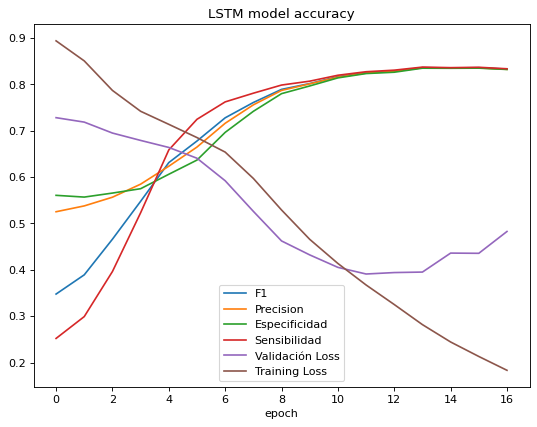
\includegraphics[scale=0.3]{D:/Q2/TFG/data/LSTM_results.png}
\end{center}

\end{figure}

Podemos observar como la sensibilidad, la especificidad, el F1 y la precisión van convergiendo hacia el 83,5\% aproximadamente. Además, vemos como el codo entre el validation loss y el training loss surge en la época 12 donde el validation loss vs training loss se comporta de forma parecida al modelo LSTM.

\subsubsection{Modelo BERT}

El modelo \hyperref[BERT_model]{BERT} ha funcionado ha funcionado significativamente mejor que los modelos anteriores. Ha obtenido, en el testing dataset, un log-loss de \textbf{0.324}, un acierto del \textbf{86,4 \%}, una sensibilidad del \textbf{86,3 \%} , una especificidad del \textbf{85,4 \%} y por tanto un F1 de \textbf{85,8 \%}. \\

El proceso de entrenamiento ha sido 4 veces más lento que el de otros modelos (alrededor de 40 segundos por época) y las métricas han convergido de la siguiente forma: 

\begin{figure}[h]
\caption{Resultados modelo BERT}
\begin{center}
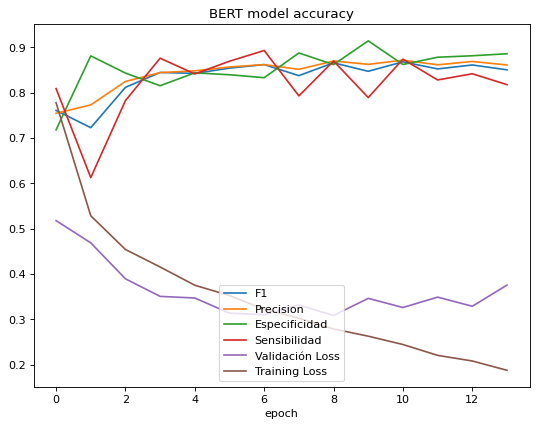
\includegraphics[scale=0.3]{D:/Q2/TFG/data/BERT_results.png}
\end{center}

\end{figure}

Podemos observar como la sensibilidad, la especificidad, el F1 y la precisión van convergiendo hacia el 86\% aproximadamente, aunque de forma más errática que en casos anteriores. Además, vemos como el codo entre el validation loss y el training loss llega hacia la época 7 donde el validation loss incrementa sobre ajustando el modelo.


\subsubsection{Modelo distilBERT}

El modelo \hyperref[distilBERT_model]{DistilBert}, como podríamos esperar, ha funcionado muy parecido al modelo BERT. Ha obtenido, en el testing dataset, un log-loss de \textbf{0.325}, un acierto del \textbf{85,6 \%}, una sensibilidad del \textbf{83,4 \%}, una especificidad del \textbf{86,3 \%}y por tanto un F1 de \textbf{84,9 \%}. \\

El proceso de entrenamiento, como avanzamos en el marco practico, ha sido un 50\% más rápido que el modelo BERT (20 segundos por época)y las métricas han convergido de la siguiente forma: 

\begin{figure}[h]
\caption{Resultados modelo distilBERT}
\begin{center}
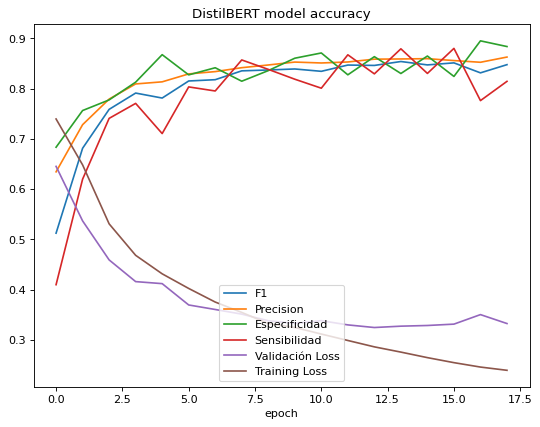
\includegraphics[scale=0.3]{D:/Q2/TFG/data/distilBERT_results.png}
\end{center}

\end{figure}

Podemos observar como la sensibilidad, la especificidad, el F1 y la precisión van convergiendo hacia el 85\% aproximadamente, aunque de forma más errática que en casos anteriores, incluyendo el modelo BERT. Además, vemos como el codo entre el validation loss y el training loss llega hacia la época 11 donde el validation loss se estanca a diferencia de los demás modelos que incrementa.

\subsubsection{Resultados globales}

Finalmente los resultados de todas las arquitecturas son los siguientes:

\begin{table}[h]
\caption{Resultados de las arquitecturas entrenadas}
\begin{tabular}{llllll}
\textbf{}           & \textbf{Loss}    & \textbf{Precisión} (\%) & \textbf{Sensibilidad} (\%) & \textbf{Especificidad} (\%) & \textbf{F1} (\%) \\ \hline
\textbf{FCNN}       & 0,363         & \hspace{0.75cm} 85,3              & \hspace{0.9cm}83,6            & \hspace{0.9cm} 85,1               & 84,4        \\
\textbf{LSTM}       & 0,369         & \hspace{0.75cm} 84,0              & \hspace{0.8cm} 84,5            & \hspace{0.9cm} 83,5               & 83,8        \\
\textbf{BERT}       & 0,324         & \hspace{0.75cm} 86,4              & \hspace{0.8cm} 86,3            & \hspace{0.9cm} 85,4               & 85,8        \\
\textbf{DistilBERT} & 0,325         & \hspace{0.75cm} 85,6              & \hspace{0.8cm} 83,4            & \hspace{0.9cm} 86,3               & 84,9       
\end{tabular}
\end{table}

Para el siguiente apartado usaremos el modelo distilBERT. Aunque no es el mejor en cuanto a resultados, si se acerca mucho y la velocidad de entrenamiento compensa la poca pérdida de rendimiento. 


\subsection{Objetivo 80\%}

Para saber que tamaño de casos sería el óptimo para este problema nos marcaremos el objetivo de llegar a un 80\% de precisión, pues el 95\% que nos propusimos al inicio es irreal. Para ello entrenaremos con diferentes proporciones del dataset de entrenamiento y analizaremos que \% de la base sería suficiente para alcanzar esta métrica. El objetivo de este ejercicio es analizar el beneficio posible que obtuviéramos si tuviéramos una base de datos con más observaciones.   

Los resultados del proceso son los siguientes:

\begin{figure}[h]
\caption{Resultados modelo distilBERT por proporción de BBDD}
\begin{center}
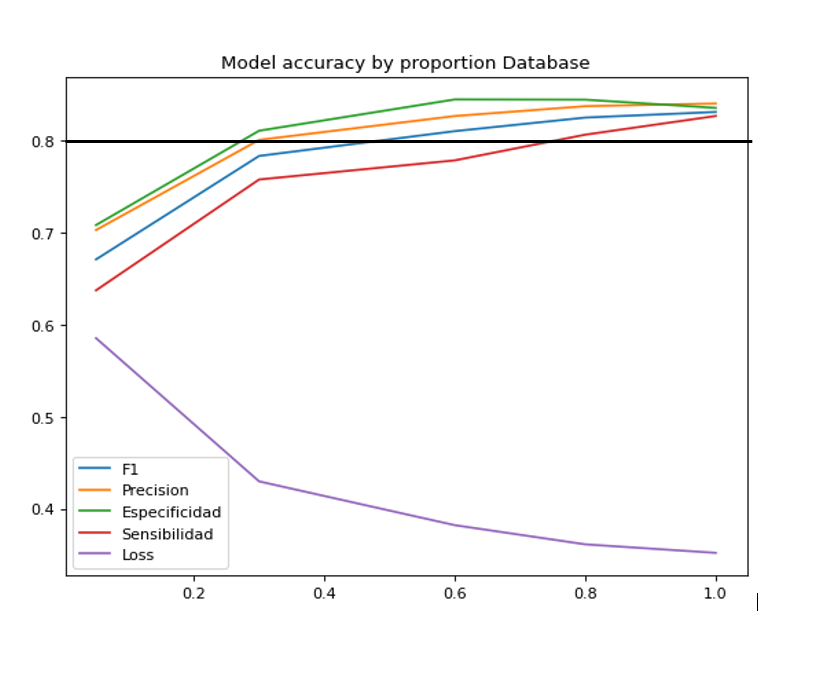
\includegraphics[scale=0.4]{D:/Q2/TFG/data/performance_80.png}
\end{center}
\end{figure}

A partir del 30\% de la base ya conseguimos un rendimiento superior al 80 \% de precisión. Esto, indica que el número de observaciones no es un problema. Sin embargo, la longitud de las frases también podría incidir en el rendimiento de las redes neuronales, especialmente BERT y distilBERT. 

\clearpage

\section{Conclusiones}

Para terminar, podemos concluir que hemos podido cumplir con todos los objetivos del trabajo. Se han entrenado los 4 modelos que nos propusimos al inicio del trabajo, teniendo en todos ellos un rendimiento más que decente (por encima del 80\% de precisión). Además, hemos conseguido ajustar los hiperparámetros del modelo mediante los datos de validación optimizando así su ajuste a los datos. Por último, hemos realizado la prueba que nos propusimos como objetivo secundario. No obstante, nuestras expectativas eran demasiados elevadas pues apuntamos a un 95\% de precisión, que, en retrospección, parece complicado con la base de datos de la que disponemos.\\ 

Cabe destacar, que en el marco práctico se ha cumplido la narrativa del marco teórico y las arquitecturas basadas en transformadores tienen mejor rendimiento que las LSTM y FCNN. Por otro lado, la diferencia de precisión entre arquitecturas es menor del esperado (1-2\%). Esto puede estar condicionado por la longitud de las frases que tenemos que clasificar, pues son muy cortas. \\


Además, podemos decir que el número de observaciones en la base es más que suficiente. Y es que reducir en un 30\% el número de observaciones de las que disponíamos solo causaba un detrimento del 5\% de precisión en el modelo distilBERT.\\

Algunas sugerencias para progresar en el análisis del sarcasmo mediante redes neuronales podrían ser: 

\begin{itemize}
\item{Analizar frases en otros idiomas.}
\item{Analizar frases de mayor longitud.}
\item{Analizar audio en vez de texto, donde la tonalidad sea un factor relevante.}
\item{Aplicar el modelo en conversaciones de texto para personas que están aprendiendo un idioma y que pueden malinterpretar algunos mensajes.}

\end{itemize}


\clearpage

\bibliographystyle{plain}
\bibliography{References}

\clearpage
\section{Annex}

\begin{lstlisting}
# -*- coding: utf-8 -*-
"""tfg-natural-language-processing.ipynb


### Import modules
"""

from google.colab import drive
drive.mount('/content/drive')

!pip install tensorflow-gpu==2.4

!pip install transformers

# pip install -q tf-models-official==2.4.0

import pandas as pd
import numpy as np
import torch
import tensorflow as tf

gpus = tf.config.experimental.list_physical_devices(device_type='GPU')
tf.config.experimental.set_visible_devices(devices=gpus[0], device_type='GPU')
tf.config.experimental.set_memory_growth(device=gpus[0], enable=True)

import seaborn as sns
import re

import wordcloud
from wordcloud import WordCloud

import matplotlib.pyplot as plt

import collections

from sklearn import preprocessing

import nltk
from nltk.corpus import stopwords
from nltk.stem import WordNetLemmatizer

import pandas as pd
import numpy as np

import matplotlib.pyplot as plt
from sklearn.model_selection import train_test_split
import time

from tensorflow.keras.preprocessing.sequence import pad_sequences

import matplotlib as mlp
import matplotlib.pyplot as plt
import seaborn as sns

from tensorflow.keras.layers import Dense, LSTM, Dropout, Embedding, GlobalMaxPool1D, Bidirectional,Input,GlobalAveragePooling1D, BatchNormalization, Conv1D,GRU
from tensorflow.keras.preprocessing.text import Tokenizer
from tensorflow.keras.utils import to_categorical
from tensorflow.keras.callbacks import EarlyStopping, ModelCheckpoint,ReduceLROnPlateau
from tensorflow.keras.models import Sequential,Model


import transformers
from transformers import AutoTokenizer,TFAutoModel, get_linear_schedule_with_warmup



"""#### Parameters

### Functions

#### Reading
"""

sarcasm_training = "/content/drive/MyDrive/TFG/data/train.csv"
sarcasm_testing = "/content/drive/MyDrive/TFG/data/test.csv"

df_training = pd.read_csv(sarcasm_training)
df_testing = pd.read_csv(sarcasm_testing)

print(df_training.columns)
print(df_training.count()) ## small dataset

df_training.isnull().sum()/df_training.count() ## no nulls

print(df_training.describe())  ## balancing data might not be a bad idea

(df_training['text'].apply(lambda x: len(str(x))) > 800).sum()

sns.boxplot(y=df_training['text'].apply(lambda x: str.split(x)).apply(lambda x: len(x))) ## about 20 words per sentence should be okay for padding

sns.boxplot(y=df_training['text'].apply(lambda x: str.split(x)).apply(lambda x: len(x) if len(x) < 140 else 10)) ## about 20 words per sentence should be okay for padding

sns.boxplot(y=df_training['text'].apply(lambda x:  len(x) if len(x) < 800 else 60))

wc1 = WordCloud(
    background_color='white', 
    max_words=100)

wc1.generate(' '.join(text for text in df_training.loc[df_training['Y'] == 1, 'text']))

plt.figure(figsize=(10,15))
plt.imshow(wc1)
plt.axis('off')
plt.title("Palabras mas comunes en frases sarcasticas")

wc = WordCloud(
    background_color='white', 
    max_words=100)

wc.generate(' '.join(text for text in df_training.loc[df_training['Y'] == 0, 'text']))

plt.figure(figsize=(10,15))
plt.imshow(wc)
plt.axis('off')
plt.title("Palabras mas comunes en frases NO sarcasticas")
plt.show()

"""### Preprocess"""

nltk.download('stopwords')

stop_words= stopwords.words('english')

def remove_stopwords(data):
    sentences=[]
    for text in data:
        text = ' '.join(word for word in text.split(' ') if word not in stop_words)
        sentences.append(text)
    return sentences

test_sentences = df_testing['text']
train_sentences = df_training['text']

test_sentences=[re.sub(r'</?a(?:(?= )[^>]*)?>',' ',frase) for frase in test_sentences]
test_sentences=[re.sub(r'[^\w\s]',' ', frase) for frase in test_sentences] 
test_sentences=[re.sub(r'\n',' ', frase) for frase in test_sentences] 

train_sentences=[re.sub(r'</?a(?:(?= )[^>]*)?>',' ',frase) for frase in train_sentences]
train_sentences=[re.sub(r'[^\w\s]',' ', frase) for frase in train_sentences] 
train_sentences=[re.sub(r'\n',' ', frase) for frase in train_sentences]

df= pd.DataFrame()
df['data'] = train_sentences
df['labels'] = df_training['Y']

y_train=to_categorical(df_training['Y'])
y_test=to_categorical(df_testing['Y'])

num_words=10000

tokenize=Tokenizer(num_words=num_words)

tokenize.fit_on_texts(train_sentences)
x_train=tokenize.texts_to_sequences(train_sentences)
x_test= tokenize.texts_to_sequences(test_sentences)

max_len = 20

x_train_pad=pad_sequences(x_train, maxlen= max_len,padding= "post")
x_test_pad=pad_sequences(x_test, maxlen= max_len, padding="post")

"""#### Definicion de arquitecturas

Primero definiremos el modelo mas simple el modelo LSTM con un embedding GloVe para agilizar el proceso de entrenamiento.
"""

embeddings_dictionary = dict()
embedding_dim = 100

# Load GloVe 100D embeddings
with open("/content/drive/MyDrive/TFG/data/glove.6B.100d.txt", encoding='utf-8') as fp:
    for line in fp.readlines():
        records = line.split()
        word = records[0]
        vector_dimensions = np.asarray(records[1:], dtype='float32')
        embeddings_dictionary [word] = vector_dimensions

vocab_length = len(tokenize.word_index) + 1
vocab_length

embedding_matrix = np.zeros((vocab_length, embedding_dim))

for word, index in tokenize.word_index.items():
    embedding_vector = embeddings_dictionary.get(word)
    if embedding_vector is not None:
        embedding_matrix[index] = embedding_vector

x_train,x_valid, y_train, y_valid = train_test_split(x_train_pad,y_train)

epochs = 20 

num_steps = epochs * len(x_train)

"""#### Red convolucional"""

from tensorflow.keras import backend as K

def custom_f1(y_true, y_pred):    
    def recall_m(y_true, y_pred):
        TP = K.sum(K.round(K.clip(y_true * y_pred, 0, 1)))
        Positives = K.sum(K.round(K.clip(y_true, 0, 1)))
        
        recall = TP / (Positives+K.epsilon())    
        return recall 
    
    
    def precision_m(y_true, y_pred):
        TP = K.sum(K.round(K.clip(y_true * y_pred, 0, 1)))
        Pred_Positives = K.sum(K.round(K.clip(y_pred, 0, 1)))
    
        precision = TP / (Pred_Positives+K.epsilon())
        return precision 
    
    precision, recall = precision_m(y_true, y_pred), recall_m(y_true, y_pred)
    
    return 2*((precision*recall)/(precision+recall+K.epsilon()))

def FCNN_NLP():
    optimizer, lr = transformers.create_optimizer(init_lr  = 2e-3, num_train_steps = num_steps,num_warmup_steps = 0.1*num_steps, weight_decay_rate =.01)



    input = Input(shape=(max_len,))
    net= (Embedding(input_dim= embedding_matrix.shape[0], output_dim= embedding_matrix.shape[1],weights=[embedding_matrix], input_length=max_len))(input)
    net = Dropout(0.2)(net)
    net = BatchNormalization()(net)
    
    net = Conv1D(32, 7, padding='same', activation='relu')(net)
    net = BatchNormalization()(net)
    net = Conv1D(32, 3, padding='same', activation='relu')(net)
    net = BatchNormalization()(net)
    net = Conv1D(32, 3, padding='same', activation='relu')(net)
    net = BatchNormalization()(net)
    net = Conv1D(32, 3, padding='same', activation='relu')(net)
    net = BatchNormalization()(net)
    
    net = Conv1D(2, 1)(net)
    net = GlobalMaxPool1D()(net)
    output = tf.keras.activations.sigmoid(net)
    model = tf.keras.models.Model(inputs = input, outputs = output)
    model.compile(optimizer=optimizer, loss='binary_crossentropy', metrics=['accuracy',tf.keras.metrics.Recall(),tf.keras.metrics.Precision(),custom_f1])
    return model
model = FCNN_NLP()
model.summary()

tf.keras.utils.plot_model(model,show_layer_names=False, rankdir = 'LR')

batch_size = 32


history = model.fit(x_train, y_train,steps_per_epoch=len(x_train)//batch_size,validation_data=(x_valid,y_valid), validation_steps=len(x_valid)//batch_size
,epochs=50, batch_size=batch_size, callbacks=[EarlyStopping(patience=5, restore_best_weights=True), ModelCheckpoint("ModelO_FCNN_checkpoint.h5", save_best_weights=True)])

tf.keras.models.save_model(model, "/content/drive/MyDrive/TFG/models/FCNN_model.h5")

FCNN_history = history

FCNN_history.history

"""#### LSTM"""

optimizer, lr = transformers.create_optimizer(init_lr  = 2e-4, num_train_steps = num_steps,num_warmup_steps = 0.1*num_steps, weight_decay_rate =.01)

model= Sequential()
    
model.add(Embedding(input_dim= embedding_matrix.shape[0], output_dim= embedding_matrix.shape[1],weights=[embedding_matrix], input_length=max_len))

model.add(tf.keras.layers.Bidirectional(LSTM(max_len, return_sequences=True))) ## if we were using a GPU backend we should remove recurrent dropout
    
model.add(GlobalMaxPool1D())
model.add(BatchNormalization())
model.add(Dropout(0.5))
model.add(Dense(max_len, activation="relu"))
model.add(Dense(max_len, activation="relu"))
    
model.add(BatchNormalization())
model.add(Dropout(0.5))
model.add(Dense(max_len, activation="relu"))
    
model.add(Dense(2, activation="softmax"))
    

model.compile(optimizer=optimizer, loss='binary_crossentropy', metrics=['accuracy',tf.keras.metrics.Recall(),tf.keras.metrics.Precision()],steps_per_execution=32)

tf.keras.utils.plot_model(model,show_layer_names=False, rankdir = 'LR')

x_train=np.array(x_train)
x_valid=np.array(x_valid)
y_train=np.array(y_train)
y_valid=np.array(y_valid)
x_test_pad= np.array(x_test_pad)
test_labels= np.array(df_testing['Y'])

history = model.fit(x_train, y_train,validation_data=(x_valid,y_valid),epochs=50, batch_size=32, callbacks=[EarlyStopping(patience=5, restore_best_weights=True), ModelCheckpoint("ModeloLSTM_embedd.h5", save_best_weights=True)])

tf.keras.models.save_model(model, "/content/drive/MyDrive/TFG/models/LSTM_model.h5")

"""#### Bert model"""

tokenizer = AutoTokenizer.from_pretrained('bert-base-cased')

X_train = np.zeros((len(df_training), max_len))
X_masks = np.zeros((len(df_training), max_len))

for i, text in enumerate(df_training['text']):
    tokens = tokenizer.encode_plus(text, max_length= max_len, \
                      truncation=True, padding = "max_length", \
                      add_special_tokens =True, return_token_type_ids = False,
                     return_attention_mask = True)
    
    X_train[i,:], X_masks[i,:] = tokens['input_ids'], tokens['attention_mask']

labels = np.array(df_training['Y'])

with open('X_train.npy','wb') as f:
    np.save(f, X_train)
with open('X_masks.npy','wb') as f:
    np.save(f, X_masks)
with open('labels.npy','wb') as f:
    np.save(f, labels)

with open('./X_train.npy','rb') as f:
    X_train = np.load(f)
with open('./X_masks.npy','rb') as f:
    X_masks = np.load(f)
with open('./labels.npy','rb') as f:
    labels = np.load(f)

X_train,X_valid,X_masks_train, X_masks_valid,labels_train,labels_valid = train_test_split(X_train,X_masks,labels)

train = tf.data.Dataset.from_tensor_slices((X_train,X_masks_train,labels_train))
validation = tf.data.Dataset.from_tensor_slices((X_valid,X_masks_valid,labels_valid))

def map_func(input_ids, masks , labels):
    return {'input_ids': input_ids, 'attention_mask':masks},labels

train = train.map(map_func)
validation = validation.map(map_func)

train = train.shuffle(1000000).batch(32)
validation = validation.shuffle(1000000).batch(32)

DS_LEN = len(list(train))

bert = TFAutoModel.from_pretrained('bert-base-cased')

input_ids = tf.keras.layers.Input(shape=(max_len,), name = 'input_ids', dtype = 'int32')
mask = tf.keras.layers.Input(shape=(max_len,), name = 'attention_mask', dtype = 'int32')

embeddings = bert(input_ids, attention_mask = mask)[0]

epochs = 50

total_steps = DS_LEN * epochs

####Try to improve this 
X = tf.keras.layers.Bidirectional(GRU(max_len, return_sequences=True))(embeddings)
X = tf.keras.layers.Dense(128, activation = 'selu')(X)
X = tf.keras.layers.Dropout(0.1)(X)
X = tf.keras.layers.Dense(128, activation = 'selu')(X)
X = tf.keras.layers.GlobalMaxPool1D()(X)
X = tf.keras.layers.Dense(128, activation = 'selu')(X)
X = tf.keras.layers.Dropout(0.3)(X)
X = tf.keras.layers.Dense(128, activation = 'selu')(X)
X = tf.keras.layers.Dropout(0.3)(X)
X = tf.keras.layers.Dense(32, activation = 'selu')(X)
y = tf.keras.layers.Dense(1, activation = 'sigmoid', name = 'outputs')(X)


model = tf.keras.Model(inputs=[input_ids, mask], outputs =y )

model.layers[2].trainable = False

tf.keras.utils.plot_model(model,show_layer_names=False,rankdir='LR')

num_steps = epochs * DS_LEN

optimizer, lr = transformers.create_optimizer(init_lr  = 8e-4, num_train_steps = num_steps,num_warmup_steps = 0.1*num_steps, weight_decay_rate =.01)

model.compile(optimizer=optimizer, loss='binary_crossentropy', metrics=['accuracy',tf.keras.metrics.Recall(),tf.keras.metrics.Precision()])

history = model.fit(train, validation_data = validation, 
                                        epochs=epochs, batch_size=32, callbacks=[EarlyStopping(patience=5, restore_best_weights=True, min_delta = 0.01), 
                                       ModelCheckpoint("ModeloBert.h5", save_best_weights=True)])

tf.keras.models.save_model(model, "/content/drive/MyDrive/TFG/models/BERT.h5")

BERT_history = history

"""#### DistilBert"""

from transformers import DistilBertTokenizer, TFDistilBertModel

tokenizer = DistilBertTokenizer.from_pretrained('distilbert-base-cased') 
distilbert = TFDistilBertModel.from_pretrained('distilbert-base-cased')

model = distilbert

X_train = np.zeros((len(df_training), max_len))
X_masks = np.zeros((len(df_training), max_len))

for i, text in enumerate(df_training['text']):
    tokens = tokenizer.encode_plus(text, max_length= max_len, \
                      truncation=True, padding = "max_length", \
                      add_special_tokens =True, return_token_type_ids = False,
                     return_attention_mask = True)
    
    X_train[i,:], X_masks[i,:] = tokens['input_ids'], tokens['attention_mask']

labels = np.array(df_training['Y'])

with open('X_train.npy','wb') as f:
    np.save(f, X_train)
with open('X_masks.npy','wb') as f:
    np.save(f, X_masks)
with open('labels.npy','wb') as f:
    np.save(f, labels)

with open('./X_train.npy','rb') as f:
    X_train = np.load(f)
with open('./X_masks.npy','rb') as f:
    X_masks = np.load(f)
with open('./labels.npy','rb') as f:
    labels = np.load(f)

X_train_source,X_masks_source,labels_source = X_train,X_masks,labels

X_train,X_valid,X_masks_train, X_masks_valid,labels_train,labels_valid = train_test_split(X_train,X_masks,labels, train_size = 0.75*prop)

train = tf.data.Dataset.from_tensor_slices((X_train,X_masks_train,labels_train))
validation = tf.data.Dataset.from_tensor_slices((X_valid,X_masks_valid,labels_valid))

def map_func(input_ids, masks , labels):
    return {'input_ids': input_ids, 'attention_mask':masks},labels

train = train.map(map_func)
validation = validation.map(map_func)

train = train.shuffle(1000000).batch(32)
validation = validation.shuffle(1000000).batch(32)

DS_LEN = len(list(train))

input_ids = tf.keras.layers.Input(shape=(max_len,), name = 'input_ids', dtype = 'int32')
mask = tf.keras.layers.Input(shape=(max_len,),name = 'attention_mask', dtype = 'int32')

embeddings = model(input_ids,attention_mask = mask)[0]

####Try to improve this 
X = tf.keras.layers.Bidirectional(LSTM(max_len, return_sequences=True))(embeddings)
X = tf.keras.layers.Dense(128, activation = 'selu')(X)
X = tf.keras.layers.GlobalMaxPool1D()(X)
X = tf.keras.layers.Dense(128, activation = 'selu')(X)
X = tf.keras.layers.Dropout(0.3)(X)
X = tf.keras.layers.Dense(128, activation = 'selu')(X)
X = tf.keras.layers.Dropout(0.3)(X)
X = tf.keras.layers.Dense(32, activation = 'selu')(X)
y = tf.keras.layers.Dense(1, activation = 'sigmoid', name = 'outputs')(X)


model = tf.keras.Model(inputs=[input_ids, mask], outputs =y )

model.layers[2].trainable = False

tf.keras.utils.plot_model(model,show_layer_names=False, rankdir= 'LR')

epochs = 50

num_steps = epochs * DS_LEN

optimizer, lr = transformers.create_optimizer(init_lr  = 8e-5, num_train_steps = num_steps,num_warmup_steps = 0.1*num_steps, weight_decay_rate =.01)
model.compile(optimizer=optimizer, loss='binary_crossentropy', metrics=['accuracy',tf.keras.metrics.Recall(),tf.keras.metrics.Precision()])

history = model.fit(train, validation_data = validation, 
                                        epochs=epochs, batch_size=32, callbacks=[EarlyStopping(patience=5, restore_best_weights=True), 
                                       ModelCheckpoint("ModeloDistilBert.h5", save_best_weights=True)])

tf.keras.models.save_model(model, "/content/drive/MyDrive/TFG/models/DistilBert.h5")

DistilBERT_history = history

"""### Evaluation"""

optimizer, lr = transformers.create_optimizer(init_lr  = 4e-5, num_train_steps = 20,num_warmup_steps = 0.1*20, weight_decay_rate =.01)

model1 = tf.keras.models.load_model('/content/drive/MyDrive/TFG/models/FCNN_model.h5', custom_objects={'AdamWeightDecay': optimizer})
model2 = tf.keras.models.load_model('/content/drive/MyDrive/TFG/models/LSTM_model.h5', custom_objects={'AdamWeightDecay': optimizer})
model3 = tf.keras.models.load_model('/content/drive/MyDrive/TFG/models/BERT.h5', custom_objects={"TFBertModel": bert,'AdamWeightDecay': optimizer})
model4 = tf.keras.models.load_model('/content/drive/MyDrive/TFG/models/DistilBert.h5', custom_objects={"TFDistilBertModel": distilbert, 'AdamWeightDecay': optimizer})

"""#### CNN evaluation"""

x = model1.evaluate(x_test_pad,y_test)

x = pd.DataFrame(x).transpose()

pd.concat((x,x), axis=0)

"""#### LSTM evaluation"""

model2.evaluate(x_test_pad,y_test)

"""#### BERT + LSTM evaluation"""

tokenizer = AutoTokenizer.from_pretrained('bert-base-cased')

X_test = np.zeros((len(df_testing), max_len))
X_test_masks = np.zeros((len(df_testing), max_len))

for i, text in enumerate(df_testing['text']):
    tokens = tokenizer.encode_plus(text, max_length= max_len, \
                      truncation=True, padding = "max_length", \
                      add_special_tokens =True, return_token_type_ids = False,
                     return_attention_mask = True)
    
    X_test[i,:], X_test_masks[i,:] = tokens['input_ids'], tokens['attention_mask']
    
test_labels = np.array(df_testing['Y'])

with open('X_test.npy','wb') as f:
    np.save(f, X_test)
with open('X_test_masks.npy','wb') as f:
    np.save(f, X_test_masks)
with open('test_labels.npy','wb') as f:
    np.save(f, test_labels)

with open('./X_test.npy','rb') as f:
    X_test = np.load(f)
with open('./X_test_masks.npy','rb') as f:
    X_test_masks = np.load(f)
with open('./test_labels.npy','rb') as f:
    test_labels = np.load(f)

dataset = tf.data.Dataset.from_tensor_slices((X_test,X_test_masks,test_labels))

def map_func(input_ids, masks , labels):
    return {'input_ids': input_ids, 'attention_mask':masks},labels

dataset = dataset.map(map_func)
dataset = dataset.shuffle(1000000).batch(32)

model3.evaluate(dataset)

"""#### Distilbert + LSTM """

tokenizer = DistilBertTokenizer.from_pretrained('distilbert-base-cased')

X_train = np.zeros((len(df_testing), max_len))
X_masks = np.zeros((len(df_testing), max_len))

for i, text in enumerate(df_testing['text']):
    tokens = tokenizer.encode_plus(text, max_length= max_len, \
                      truncation=True, padding = "max_length", \
                      add_special_tokens =True, return_token_type_ids = False,
                     return_attention_mask = True)
    
    X_test[i,:], X_test_masks[i,:] = tokens['input_ids'], tokens['attention_mask']
    
test_labels = np.array(df_testing['Y'])

with open('X_test.npy','wb') as f:
    np.save(f, X_test)
with open('X_test_masks.npy','wb') as f:
    np.save(f, X_test_masks)
with open('test_labels.npy','wb') as f:
    np.save(f, test_labels)

with open('./X_test.npy','rb') as f:
    X_test = np.load(f)
with open('./X_test_masks.npy','rb') as f:
    X_test_masks = np.load(f)
with open('./test_labels.npy','rb') as f:
    test_labels = np.load(f)

dataset = tf.data.Dataset.from_tensor_slices((X_test,X_test_masks,test_labels))

def map_func(input_ids, masks , labels):
    return {'input_ids': input_ids, 'attention_mask':masks},labels

dataset = dataset.map(map_func)
dataset = dataset.shuffle(1000000).batch(32)

model4.evaluate(dataset)



"""#### Visualization validation"""

F1_FCNN = list(2*np.array(FCNN_history.history['val_precision_6'])*np.array(FCNN_history.history['val_recall_6'])/(np.array(FCNN_history.history['val_precision_6'])+ np.array(FCNN_history.history['val_recall_6'])))

from matplotlib import pyplot as plt
from matplotlib.pyplot import figure

figure(figsize=(8, 6), dpi=80)


plt.plot(F1_FCNN)
plt.plot(FCNN_history.history['val_accuracy'])
plt.plot(FCNN_history.history['val_precision_6'])
plt.plot(FCNN_history.history['val_recall_6'])
plt.plot(FCNN_history.history['val_loss'])
plt.plot(FCNN_history.history['loss'])
plt.title('FCNN model accuracy')
plt.xlabel('epoch')
plt.legend(["F1",'Precision','Especificidad', 'Sensibilidad','Validacion Loss','Training Loss'], loc='lower center')
plt.show()

F1_LSTM= list(2*np.array(LSTM_history.history['val_precision_10'])*np.array(LSTM_history.history['val_recall_10'])/(np.array(LSTM_history.history['val_precision_10'])+ np.array(LSTM_history.history['val_recall_10'])))

from matplotlib import pyplot as plt
from matplotlib.pyplot import figure

figure(figsize=(8, 6), dpi=80)

plt.plot(F1_LSTM)
plt.plot(LSTM_history.history['val_accuracy'])
plt.plot(LSTM_history.history['val_precision_10'])
plt.plot(LSTM_history.history['val_recall_10'])
plt.plot(LSTM_history.history['val_loss'])
plt.plot(LSTM_history.history['loss'])
plt.title('LSTM model accuracy')
plt.xlabel('epoch')
plt.legend(['F1','Precision','Especificidad', 'Sensibilidad','Validacion Loss','Training Loss'], loc='lower center')
plt.show()

F1_BERT= list(2*np.array(BERT_history.history['val_precision_11'])*np.array(BERT_history.history['val_recall_11'])/(np.array(BERT_history.history['val_precision_11'])+ np.array(BERT_history.history['val_recall_11'])))

from matplotlib import pyplot as plt
from matplotlib.pyplot import figure

figure(figsize=(8, 6), dpi=80)


plt.plot(F1_BERT)
plt.plot(BERT_history.history['val_accuracy'])
plt.plot(BERT_history.history['val_precision_11'])
plt.plot(BERT_history.history['val_recall_11'])
plt.plot(BERT_history.history['val_loss'])
plt.plot(BERT_history.history['loss'])
plt.title('BERT model accuracy')
plt.xlabel('epoch')
plt.legend(['F1','Precision','Especificidad', 'Sensibilidad','Validacion Loss','Training Loss'], loc='lower center')
plt.show()

F1_distilBERT= list(2*np.array(DistilBERT_history.history['val_precision_12'])*np.array(DistilBERT_history.history['val_recall_12'])/(np.array(DistilBERT_history.history['val_precision_12'])+ np.array(DistilBERT_history.history['val_recall_12'])))

from matplotlib import pyplot as plt
from matplotlib.pyplot import figure

figure(figsize=(8, 6), dpi=80)

plt.plot(F1_distilBERT)
plt.plot(DistilBERT_history.history['val_accuracy'])
plt.plot(DistilBERT_history.history['val_precision_12'])
plt.plot(DistilBERT_history.history['val_recall_12'])
plt.plot(DistilBERT_history.history['val_loss'])
plt.plot(DistilBERT_history.history['loss'])
plt.title('DistilBERT model accuracy')
plt.xlabel('epoch')
plt.legend(['F1','Precision','Especificidad', 'Sensibilidad','Validacion Loss','Training Loss'], loc='lower center')
plt.show()

"""#### Objetivo 80% """

from transformers import DistilBertTokenizer, TFDistilBertModel

tokenizer = DistilBertTokenizer.from_pretrained('distilbert-base-cased') 
distilbert = TFDistilBertModel.from_pretrained('distilbert-base-cased')

model = distilbert
max_len =20

X_train = np.zeros((len(df_training), max_len))
X_masks = np.zeros((len(df_training), max_len))

for i, text in enumerate(df_training['text']):
    tokens = tokenizer.encode_plus(text, max_length= max_len, \
                      truncation=True, padding = "max_length", \
                      add_special_tokens =True, return_token_type_ids = False,
                     return_attention_mask = True)
    
    X_train[i,:], X_masks[i,:] = tokens['input_ids'], tokens['attention_mask']

labels = np.array(df_training['Y'])

with open('X_train.npy','wb') as f:
    np.save(f, X_train)
with open('X_masks.npy','wb') as f:
    np.save(f, X_masks)
with open('labels.npy','wb') as f:
    np.save(f, labels)

with open('./X_train.npy','rb') as f:
    X_train = np.load(f)
with open('./X_masks.npy','rb') as f:
    X_masks = np.load(f)
with open('./labels.npy','rb') as f:
    labels = np.load(f)

X_test = np.zeros((len(df_testing), max_len))
X_test_masks = np.zeros((len(df_testing), max_len))

for i, text in enumerate(df_testing['text']):
    tokens = tokenizer.encode_plus(text, max_length= max_len, \
                      truncation=True, padding = "max_length", \
                      add_special_tokens =True, return_token_type_ids = False,
                     return_attention_mask = True)
    
    X_test[i,:], X_test_masks[i,:] = tokens['input_ids'], tokens['attention_mask']
    
test_labels = np.array(df_testing['Y'])

with open('X_test.npy','wb') as f:
    np.save(f, X_test)
with open('X_test_masks.npy','wb') as f:
    np.save(f, X_test_masks)
with open('test_labels.npy','wb') as f:
    np.save(f, test_labels)

with open('./X_test.npy','rb') as f:
    X_test = np.load(f)
with open('./X_test_masks.npy','rb') as f:
    X_test_masks = np.load(f)
with open('./test_labels.npy','rb') as f:
    test_labels = np.load(f)

test_dataset = tf.data.Dataset.from_tensor_slices((X_test,X_test_masks,test_labels))

def map_func(input_ids, masks , labels):
    return {'input_ids': input_ids, 'attention_mask':masks},labels

test_dataset = test_dataset.map(map_func)
test_dataset = test_dataset.shuffle(1000000).batch(32)

X_train_source = X_train
X_masks_source = X_masks
labels_source = labels

results = [0,0,0,0]
results = pd.DataFrame(results).transpose()

for prop in [0.05,0.3,0.6, 0.8,1]:
  X_train,X_valid,X_masks_train, X_masks_valid,labels_train,labels_valid = train_test_split(X_train_source,X_masks_source,labels_source, train_size = 0.75*prop)

  train = tf.data.Dataset.from_tensor_slices((X_train,X_masks_train,labels_train))
  validation = tf.data.Dataset.from_tensor_slices((X_valid,X_masks_valid,labels_valid))

  def map_func(input_ids, masks , labels):
      return {'input_ids': input_ids, 'attention_mask':masks},labels

  train = train.map(map_func)
  validation = validation.map(map_func)

  train = train.shuffle(1000000).batch(32)
  validation = validation.shuffle(1000000).batch(32)

  DS_LEN = len(list(train))

  input_ids = tf.keras.layers.Input(shape=(max_len,), name = 'input_ids', dtype = 'int32')
  mask = tf.keras.layers.Input(shape=(max_len,),name = 'attention_mask', dtype = 'int32')

  embeddings = distilbert(input_ids,attention_mask = mask)[0]


  ####Try to improve this 
  X = tf.keras.layers.Bidirectional(LSTM(max_len, return_sequences=True))(embeddings)
  X = tf.keras.layers.Dense(128, activation = 'selu')(X)
  X = tf.keras.layers.GlobalMaxPool1D()(X)
  X = tf.keras.layers.Dense(128, activation = 'selu')(X)
  X = tf.keras.layers.Dropout(0.3)(X)
  X = tf.keras.layers.Dense(128, activation = 'selu')(X)
  X = tf.keras.layers.Dropout(0.3)(X)
  X = tf.keras.layers.Dense(32, activation = 'selu')(X)
  y = tf.keras.layers.Dense(1, activation = 'sigmoid', name = 'outputs')(X)


  model = tf.keras.Model(inputs=[input_ids, mask], outputs =y )

  model.layers[2].trainable = False


  epochs = 20

  num_steps = epochs * DS_LEN

  optimizer, lr = transformers.create_optimizer(init_lr  = 4e-5, num_train_steps = num_steps,num_warmup_steps = 0.1*num_steps, weight_decay_rate =.01)
  model.compile(optimizer=optimizer, loss='binary_crossentropy', metrics=['accuracy',tf.keras.metrics.Recall(),tf.keras.metrics.Precision()])


  model.fit(train, validation_data = validation, 
                                          epochs=epochs, batch_size=32, callbacks=[EarlyStopping(patience=3, restore_best_weights=True), 
                                        ModelCheckpoint("ModeloDistilBert.h5", save_best_weights=True)])

  x = model.evaluate(test_dataset)
     
  x = pd.DataFrame(x).transpose()

  results = pd.concat((results,x), axis=0)

results = results.iloc[1:,]

results.columns = ['Loss','Precision','Sensibilidad','Especificidad']

results['Proporcion'] = [0.05,0.3,0.6, 0.8,1]

results['F1'] = (2*results['Especificidad']*results['Sensibilidad'])/(results['Especificidad']+results['Sensibilidad'])

from matplotlib import pyplot as plt
from matplotlib.pyplot import figure

figure(figsize=(8, 6), dpi=80)


plt.plot(results['F1'])
plt.plot(results['Precision'])
plt.plot(results['Especificidad'])
plt.plot(results['Sensibilidad'])
plt.plot(results['Loss'])
plt.title('Model accuracy by proportion Database')
plt.legend(["F1",'Precision','Especificidad', 'Sensibilidad','Loss'], loc='Best')
plt.show()


\end{lstlisting}


\end{document}

